%        File: VTthesis_template.tex
%     Created: Thu Mar 24 11:00 AM 2016 EDT
%     Last Change: Mon, April 30, 2018
%      Author: Alan M. Lattimer, VT
%	   With modifications by Carrie Cross, Robert Browder, and LianTze Lim.
%
% This template is designed to operate with XeLaTeX.
%
% All elements in the Title, Abstract, and Keywords MUST be formatted as text and NOT as math.
%
%Further instructions for using this template are embedded in the document. Additionally, there are comments at the end of the file that give suggestions on writing your thesis.
%
%In addition to the standard formatting options, the following options are defined for the VTthesis class: proposal, prelim, doublespace, draft.

\documentclass[nopageskip,prelim]{VTthesis} % nopageskip = Removes arbitrary blank pages.

\usepackage{microtype} % Not everything is supported when using XeLaTeX, but should help a bit in making text look nicer.
\usepackage{textcomp}  % Fixes issue with microtype+siunitx's \micro

\usepackage[en-US]{datetime2}      % For \DTMdate, etc.
\usepackage[binary-units]{siunitx}
\usepackage{mathtools}             % for \coloneqq
\usepackage{bussproofs}            % for prooftree environment

\usepackage{booktabs}              % For nicer-looking tables
\usepackage{makecell}              % For table heading cells and cells with line breaks
\usepackage{threeparttable}        % For tables with notes
\usepackage[inline]{enumitem}

\usepackage[index,single]{acro}                  % For acronyms; hyperref option changes acro colors but doesn't actually link to the list so not using it right now
\usepackage{makeidx}               % For indices!

\usepackage{pgfplots}               % For plots

\usetikzlibrary{external}          % To reduce build times for complex figures (does one-time builds and stores as images)
\usetikzlibrary{graphs}            % dot-style graph shorthands (not quite as compactible as dot language, though)
\usetikzlibrary{quotes}            % needed for quoted edge labels (only in graphs?)

\pgfplotsset{compat=1.15}          % For up-to-date features
\tikzexternalize[prefix=extern/]                  % Enables externalization (has issues with figures containing references when used with XeLaTeX, so turn off externalization when you need those)

\renewcommand\lstlistlistingname{List of Listings}

\DeclareAcronym{abi}{
  short            = ABI,
  short-indefinite = an,
  long             = application binary interface,
  long-indefinite  = an
}
\DeclareAcronym{aec2}{short=Amazon EC2, long=Amazon Elastic Compute Cloud}
\DeclareAcronym{afp}{short=AFP, long=Archive of Formal Proofs}
\DeclareAcronym{cfg}{short=CFG, long=control flow graph}
\DeclareAcronym{cfi}{short=CFI, long=control-flow integrity}
\DeclareAcronym{dm}{short=DM, long=device model}
\DeclareAcronym{fmuc}{
  short            = FMUC,
  short-indefinite = an,
  long             = formal memory usage certificate
}
\DeclareAcronym{hvm}{
  short            = HVM,
  short-indefinite = an,
  long             = hardware virtual machine
}
\DeclareAcronym{gcc}{short=GCC, long=the GNU Compiler Collection}
\DeclareAcronym{icc}{
  short            = ICC,
  short-indefinite = an,
  long             = the Intel C++ Compiler
}
\DeclareAcronym{ipc}{
  short            = IPC,
  short-indefinite = an,
  long             = inter-process communication,
  long-indefinite  = an
}
\DeclareAcronym{isa}{
  short            = ISA,
  short-indefinite = an,
  long             = instruction set architecture,
  long-indefinite  = an
}
\DeclareAcronym{itp}{
  short            = ITP,
  short-indefinite = an,
  long             = interactive theorem proving,
  long-indefinite  = an
}
\DeclareAcronym{mrr}{short=MRR, long=memory region relation}
\DeclareAcronym{os}{
  short            = OS,
  short-indefinite = an,
  long             = operating system,
  long-indefinite  = an,
  short-plural     = es
}
\DeclareAcronym{qemu}{short=QEMU, long=Quick Emulator}
\DeclareAcronym{scf}{
  short            = SCF,
  short-indefinite = an,
  long             = syntactic control flow
}
\DeclareAcronym{simd}{short=SIMD, long=single instruction multiple data}
\DeclareAcronym{sloc}{short=SLOC, long=source lines of code}
\DeclareAcronym{smt}{
  short            = SMT,
  short-indefinite = an,
  long             = satisfiability modulo theories
}
\DeclareAcronym{sse}{
  short            = SSE,
  short-indefinite = an,
  long             = Streaming SIMD Extensions,
  long-indefinite  = an,
}
\DeclareAcronym{tcb}{short=TCB, long=trusted computing base}
\DeclareAcronym{vm}{short=VM, long=virtual machine}
\DeclareAcronym{vmm}{short=VMM, long=virtual machine monitor}

\lstdefinelanguage
  [x64]{Assembler}     % add an "x64" dialect of Assembler
  [x86masm]{Assembler} % based on the "x86masm" dialect
  % with these extra keywords:
  {morekeywords={CDQE,CQO,CMPSQ,CMPXCHG16B,JRCXZ,LODSQ,MOVSXD,% will add more insts as needed
      POPFQ,PUSHFQ,SCASQ,STOSQ,IRETQ,RDTSCP,SWAPGS,%
      MOVAPD,MOVDQA,
      dil,%
      rax,rdx,rcx,rbx,rsi,rdi,rsp,rbp,rip,%
      r8,r8d,r8w,r8b,r9,r9d,r9w,r9b,%
      r10,r10d,r10w,r10b,r11,r11d,r11w,r11b,%
      r12,r12d,r12w,r12b,r13,r13d,r13w,r13b,%
      r14,r14d,r14w,r14b,r15,r15d,r15w,r15b}} % etc.
\lstdefinestyle{x64}{
  language=[x64]{Assembler},
  keywordstyle=\bfseries\color{blue}, % bold blue keywords
  commentstyle=\color{gray},
  identifierstyle=\color{purple},
  stringstyle=\color{brown},
}

\newcommand{\xenpercentage}{\SI{71}{\percent}}
\newcommand{\xenpercentagenot}{\SI{29}{\percent}}

\newcommand{\inlineasm}[1]{\lstinline[style=x64]|#1|}

%% Math commands
\newcommand{\var}[1]{\mathit{#1}}
\DeclareMathOperator{\step}{step}
\DeclareMathOperator{\run}{run\_until}
\DeclareMathOperator{\loc}{loc}
\DeclareMathOperator{\rbxpops}{multiplicands\_pushed}
\DeclareMathOperator{\retsites}{ret\_addrs\_pushed}

\newcommand{\region}[2]{\ensuremath{[#1,#2]}}
\newcommand{\readmem}[2]{\ensuremath{\ast\region{#1}{#2}}}
\newcommand{\readmemS}[3]{\ensuremath{#1:\readmem{#2}{#3}}}
\newcommand{\htriple}[3]{\{#1\}~#2~\{#3\}}
\newcommand{\parent}[3]{\operatorname{parent}(#1,#2,#3)}

\newcommand{\deqptr}{\var{deq}_\mathrm{ptr}}
\newcommand{\bufferptr}{\var{buf}_\mathrm{ptr}}
\newcommand{\outptr}{\var{out}_\mathrm{ptr}}
\newcommand{\valueptr}{\var{value}_\mathrm{ptr}}

\newcommand{\mathrip}{\text{\inlineasm{rip}}}
\newcommand{\mathrbp}{\text{\inlineasm{rbp}}}
\newcommand{\mathrbx}{\text{\inlineasm{rbx}}}
\newcommand{\mathrdi}{\text{\inlineasm{rdi}}}
\newcommand{\mathrsi}{\text{\inlineasm{rsi}}}
\newcommand{\mathrsp}{\text{\inlineasm{rsp}}}
\newcommand{\mathdil}{\text{\inlineasm{dil}}}
\newcommand{\mathdl}{\text{\inlineasm{dl}}}

\newcommand{\rspo}{\var{rsp}_0}
\newcommand{\rbpo}{\var{rbp}_0}

\newcommand{\retaddr}{\mathtt{ret\_addr}}

% Misc. commands
\newcommand{\todo}[1]{{\bfseries\color{purple}#1}} % Allowing paragraphs in todos
\newcommand*{\fturl}[1]{\footnote{\url{#1}}}

% Title of your thesis
\title{Title of your thesis goes here}

% You should include 3-5 keywords, separated by commas
\keywords{Some Keywords, Subject matter, etc.}

\author{Joshua A. Bockenek}
\program{Electrical and Computer Engineering}
\degree{Doctor of Philosophy}

% This should be your defense date: (update when settled)
\submitdate{\DTMdate{2019-09-01}}

\principaladvisor{Binoy Ravindran}
\firstreader{Freek Verbeek}
\secondreader{Patrick R. Schaumont}
\thirdreader{Michael S. Hsiao}
\fourthreader{Changhee Jung}
%\fifthreader{}

% The dedication and acknowledgement pages are optional. Comment them out to remove them.
\dedication{This is where you put your dedications.}
\acknowledge{This is where you put your acknowledgments.}

% The abstract is required and should be <=250 words for thesis, <=350 words for dissertation.
\abstract{Give a brief description of your thesis here. Max of 250 words for a master's thesis and 350 words for a PhD dissertation, according to the VT ETD standards.}

% The general audience abstract is required. There are currently no word limits.
\abstractgenaud{You are also required as of Spring 2016 to include a general audience abstract. This should be geared towards individuals outside of your field that may be reading seeking information about your work. You should avoid language that is particular to your field and clearly define any terms that may have special meaning in your discipline.}

\makeindex
\begin{document}
  \frontmatter
  \maketitle
  \tableofcontents

	\listoffigures
  \listoftables
  % Bit of work needed to get listings and acronyms in the TOC properly
  \clearpage\phantomsection % Getting hyperref to link to the right page
  \addcontentsline{toc}{chapter}{\lstlistlistingname}
  \lstlistoflistings
  \clearpage\phantomsection % Getting hyperref to link to the right page
  \addcontentsline{toc}{chapter}{Acronyms}
  \printacronyms[heading=chapter*]
  \printnomenclature

  % The following sets up the document for the main part of the thesis or dissertation. Do not comment out or remove this line.
	\mainmatter

  \chapter{Introduction}
Proving that a non-trivial program has no bugs is not an easy task,
and as technology continues to improve,
software will continue to increase in complexity.
Providing methods to ease the work of reasoning over programs is a necessity
in the modern world.
This is particularly important for programs
that are intended for high-reliability applications,
such as avionics or medical equipment.

\section{Motivation}
Using formal, mathematical techniques to reason about and prove properties of programs
greatly increases their reliability and trustworthiness.
The downside is the high degree of effort required to achieve that level of reliability.
Achieving reasonable formal analyses without requiring an excessive degree of effort
would surely encourage more people to use those analyses.

As an example, several years ago Facebook integrated the static analysis tool Infer
into their \ac{ci} toolchain \autocite{calcagno2011infer}.
That tool, which uses formal techniques to identify potential bugs
that other static analysis tools may not detect,
requires minimal user interaction to function.
If this could be done with more forms of formal analysis,
it would make the world of software development a better place.

While formal methods are not yet widely used in industry outside of hardware design
and other applications requiring the highest level of security,
the world does seem to be slowly moving in that direction
\autocite{smackers2019,khazeev2019acceptance}.
Putting in the work to increase their automation and usability
would have advantages beyond just the research community.

\subsection{Importance}
Increasing complexity in software development makes programs harder to reason about.
Sir Charles Antony Richard Hoare
once bemoaned the state of software development in his time \autocite{hoare1980clothes},
the favoring of adding fancy language features over minimizing the possibility of bugs.
To quote him:
\begin{quote}
  There is nothing a mere scientist can say that will stand against the flood
  of a hundred million dollars. But there is one quality that cannot be purchased
  in this way---and that is reliability. The price of reliability is the pursuit of
  the utmost simplicity. It is a price which the very rich find most hard to pay.
\end{quote}
This was said almost forty years ago, but things do not seem to have changed much.
The recent debacles with Meltdown and Spectre  \autocite{lipp2018meltdown,kocher2018spectre}
are yet another case of a push for additional performance having unexpected,
negative consequences.
Admittedly, those were hardware rather than software issues,
but in a way that is even worse. Once identified, a software problem can be resolved
with an update or patch, but hardware issues are much harder to fix.

Ultimately, given how modern life involves being surrounded by devices
running all kinds of software, there is a need for accurate analysis
of the properties of the programs we use in our everyday lives.
\Ac{iot} devices in particular have not had a particularly good reputation
when it comes to security \autocite{zhang2014iot,zhao2013iot}, despite their popularity.
Lowering the bar for verifying the safety and security of everyday devices
would improve quality of life and grant greater peace of mind.

\subsection{Challenges}
Highly-automated verification efforts are desirable, but do not necessarily scale.
Model checking, in particular, suffers from what is known as the
``state explosion'' problem \autocite{clarke2012modelchecking}.
Though there have been significant improvements in model-checking performance
in the past decades, model checkers still have issues with large, complex systems.

On the opposite side of the interactivity level is \emph{\ac{itp}}.
Interactive theorem provers and proof assistants
like Isabelle/HOL \autocite{nipkow2002isabelle}, Coq \autocite{chlipala2013certified},
and HOL4  \autocite{slind2008brief} are powerful tools for producing meaningful proofs.
Unfortunately, their learning curves are not exactly flat.
The average software developer will not want to have to spend the time
learning how to write formal proofs just to eliminate some bugs from their programs.

Targeting an approach somewhere in the middle,
automating the bulk of the proof effort while still allowing user interaction,
may be the best way to go.
This does require a significant amount of up-front verification work, however.
Developing a proof-generation framework that allows easy interaction
without the need for any in-depth work is pretty much impossible.
The most that can be achieved is a minimization of the work needed.
With the right properties chosen, however, it is possible to greatly minimize that work.

Choosing those properties wisely can even allow significant verification effort
on the \emph{assembly level}.

\section{Assembly-Level Verification}
There are many approaches for formal verification that target source code
and higher level languages in general.
This dissertation, however, focuses on \emph{assembly-level} verification.

Targeting assembly means that there is no need to trust all the steps between
writing source code and obtaining a binary from it.
Doing so reduces the \ac{tcb} without needing to use a compiler
that has been formally proven to maintain the semantics of the source code
in the binaries it produces. On the flip side, analyzing code on the assembly level
is harder than analyzing source code.
While the individual instructions are usually simpler
than any individual higher-level statement could be,
there are a lot more of them and they lack some of the abstraction
that can help simplify reasoning on a higher level. \Cref{asm_challenges}
covers some of the issues with verification on the assembly level.

Even so, there are properties that can only be identified on the assembly level
due to how close assembly is to the machine it is executed on,
as detailed in the following section.

\subsection{Importance}
Properties that reason over the concrete memory used by a program
cannot be satisfactorily expressed on the source-code level.
This is because even programs in a relatively low-level language like C
have abstractions on memory for local variables and function calls.
How and where that memory is allocated may be compiler, \ac{abi}, and \ac{isa}-specific.
It can even depend on what compiler options are in use,
including the level of optimization.
While one way of resolving that issue would be to choose a specific compiler
and provide a formal analysis of how it arranges memory (or write a compiler to do so),
that method places restrictions on the build process.
Targeting assembly or machine code directly, as done in this dissertation,
allows bypassing the build process, opening the door for verification of legacy code.
\begin{example}\label{ex:rop}
  As a further illustration, consider formulating a property
  that a function cannot overwrite its own return address.
  Doing so would require knowledge of the layout of the stack,
  including the values of the stack and frame pointers,
  thus making it an \emph{assembly-level} property.
\end{example}

\subsection{Challenges}\label{asm_challenges}
The biggest challenge in assembly-level verification is
the semantic gap between compiled and source code.
Higher-level languages hide details of their implementation
behind layers of abstraction, which makes it easier to reason about them on that level
but makes it harder to formally show equivalence with the semantics of
to lower abstraction levels.
Meanwhile, assembly languages are close to direct interfaces
with their corresponding \acp{isa},
having minimal differences in semantics but not being easy to reason about directly.

As an example of the semantic gap,
assembly code generally lacks the structured control flow found in languages
on a higher level of extraction.
Instead, all control flow on the assembly level is performed using conditional
or unconditional branches, either to a predetermined location
or to a calculated label.

A further example would be source code containing division operations
being compiled to run on a processor that does not provide hardware division.
Many \acp{cpu} for embedded systems lack support for hardware division
as efficient division algorithms require a lot of circuitry.
For such processors, runtime division must be calculated using an algorithm
implemented in assembly rather than via a specific instruction.

Even the basic concept of numeric types is minimal on the assembly level,
much less more abstract data types like lists or trees.
While most \acp{isa} do have different instructions
for signed versus unsigned integer arithmetic,
as well as distinct instructions for floating-point operations,
individual values in memory have no type.
They are merely lists of bytes starting at some address,
and even the number of bytes and the address to read from or write to can be variable.
A user could go as far as supplying the result of a floating-point computation
as the address operand of an instruction that loads or stores memory.
Historically, there have been computers that associated type information
with memory locations in hardware \autocite{feustel1972rice,feustel1973advantages,thornton2008rice},
but we do not have that luxury on typical modern systems.

An additional issue with assembly,
and the one most significant for this dissertation,
lies in the simplicity of the user-exposed memory model.
The vast majority of high-level, structured languages with scoping
prevent function calls from accessing the local variables of other calls
without significant effort or explicit notation, but the same is not true for assembly.
An assembly instruction that operates on memory can refer to any
address within range of its address operands even if it is not supposed to.
Most modern \acp{isa} do provide some form of memory protection,
but those generally rely on runtime detection of invalid accesses
and are often not fine-grained enough for reasoning about individual stack frames
or local variables.
Any verification effort that wishes to reason about low-level memory properties
must provide its own abstractions and assumptions on layout.

\subsection{Current Approaches to Assembly Verification}
A few years ago, \textcite{tan2015auspice} introduced a logic framework called AUSPICE
for automated verification of safety properties on the assembly level.
That work took six hours to execute on \num{533} instructions,
but was applicable to unmodified code.

A little before that, \textcite{shi2012orientais} provided a verification methodology
for a real-time \ac{os} designed for automotive applications.
Part of their verification methodology involved lifting machine code into an intermediate
representation called xBIL \autocite{shi2012xbil}.

More recently, \textcite{baumann2016high} provided an ARMv8-based hypervisor
that was formally verified on the machine code level
to ensure isolation of guest \acp{os}.
That work was based on an earlier one for an ARMv7 separation kernel,
PROSPER \autocite{dam2013hypervisor,dam2013formal}.

Around the same time, \textcite{goel2014syscalls,goelphd} produced formal semantics
for most user-mode x86-64 instructions as well as for commonly-used system calls.
Their work allows mechanized reasoning over compiled programs
in the ACL2 theorem prover \autocite{ACL2}.

Additionally, earlier this year, \textcite{fromherz2019verified} embedded a subset
of the x86-64 \ac{isa} in the functional, verification-oriented language
F$^*$ \autocite{fstar}.
This was done in order to perform a proof of correctness
over the commonly-used cryptographic routine AES-GCM.

\section{Research Contributions}
This dissertation presents two formal approaches to function-oriented verification
of the assembly-level property we call \emph{memory preservation},
described in \cref{memory_usage}:
\emph{control-flow-driven} verification and \emph{syntax-driven} verification.
Both approaches use some form of control-flow analysis over functions in x86-64 assembly
to generate incomplete proofs.
Those proofs are then loaded into the interactive theorem prover Isabelle/HOL
and completed there. The proof strategies for both approaches involve
\emph{symbolic execution} of the underlying assembly code \autocite{king1976symbolic},
albeit in different ways.

The main differences between the two approaches
lie in their degrees of automation, the strengths of their invariants,
and how they perform symbolic execution.
The first approach, control-flow-driven verification,
requires significantly more user user input but has the potential for much stronger invariants.
Meanwhile, the second approach, syntax-driven verification,
has a significantly higher level of proof automation
but is not as suited for stronger invariant production.
Symbolic execution is also more efficient in the control-flow-driven approach
as it more closely follows the structure of the function \ac{cfg}.
In contrast, the syntax-driven approach must deal with
operating on a restricted set of control flow constructs,
which can result in extra symbolic execution.

\subsection{Memory Usage and Preservation}\label{memory_usage}
\emph{Memory usage} characterizes the regions in memory that are read and written by a program.
An extension of memory usage is the property of \emph{memory preservation},
which states that the values written by that program are constrained to those memory regions.
The following sections elaborate on the usefulness of memory preservation
as a platform for further verification efforts,
after which the control-flow-driven and syntax-driven methodologies are discussed further.

\subsubsection{Security}
Unbounded memory usage can lead to vulnerabilities
such as buffer overflows and data leakage.
One example of such a vulnerability would be 2014's Heartbleed \autocite{heartbleed}.
Heartbleed was caused by a lack of bounds checking on a string array
requested as output as part of a ``heartbeat'' message.
This, combined with a custom memory manager
that also had no security protections against out-of-bounds memory accesses,
lead to potential leakage of sensitive data such as passwords and encryption keys.
Memory preservation could serve as a foundation for formal security analyses
that could be used to expose vulnerabilities involving malicious writes.

Another important property that memory preservation could help with
is \emph{\ac{cfi}} \autocite{abadi2009cfi}. \Ac{cfi} ensures that software execution
follows a predetermined \ac{cfg} using static analysis and runtime checks.
The dynamic checking could be made more efficient
by first proving the property in \cref{ex:rop} for those functions it is applicable to
and then leaving out any return-oriented checks for those functions it holds on.
This could be one way of avoiding \ac{rop} attacks without excessive runtime overhead.

The property of \emph{noninterference} is also a useful one for security.
It requires reasoning over which parts of the memory are used by which functions \autocite{rushby1992noninterference},
and memory preservation is ideal for such a scenario.

\subsubsection{Composition}\label{sse:composition}
Scalability in verification is only feasible with composition;
proofs of functional correctness or some other property over a large suite of software
require decomposing that suite into manageable chunks.
Separation logic provides a \emph{frame rule} that supports such%
\index{separation logic!frame rule}
decomposition \autocite{o2001local,reynolds2002separation,krebbers2017essence}.
In words, the frame rule states that,
if a program or program fragment can be confined to a certain part of a state,
properties of that program or program fragment carry over
when used as part of a larger system involving that state.
Memory preservation allows for discharging the most involved part of the frame rule,
at least in terms of individual assembly functions.
That is, it shows that the memory preservation of those functions is constrained
to specific regions in memory.
This could then serve as a basis
for a larger proof effort over multi-function assembly programs.

\subsubsection{Concurrency}
Reasoning over concurrent programs is complicated
due to the potential interactions between threads.
While there are ways of handling such interactions in a structured manner
via kernel- or library-provided \ac{ipc},
one method commonly used for the sake of efficiency is \emph{shared memory}.
Shared memory, in the context of this work,
refers to threads or processes sharing either a full memory space
or portions of one (via memory mapping)
that can be written to and read from freely by any thread or process with access to it.
Usage of shared memory can result in \emph{unintended} interactions between threads.
Memory preservation could be adapted to show the absence of such interactions
by proving that multiple threads only write
to specifically-allowed regions of shared memory.
Doing so would, of course, require a proper model of concurrency,
which is out of scope of this dissertation.

\subsection{Control-Flow-Driven Verification}
This methodology for verification of memory preservation relies on treating function bodies
as \acp{cfg} with basic blocks as the nodes, much as compilers do when performing their analyses.
In order to reason about the \acp{cfg},
they are annotated with predicates on state at specific locations,
between which the program will be symbolically executed.
While it is possible to reason about full functional correctness with this methodology,
doing so takes a significant amount of effort due to the very low level of abstraction
assembly provides, even with proven-correct formal simplification rules in Isabelle.
Because of this, we focused on the aforementioned property of memory preservation.

%Formal Definition of Memory Preservation
In our model, memory usage is formulated as a set of \emph{regions}
that start at some address and have a specific size in bytes.
We do not currently differentiate between regions for writes and regions for reads,
though doing so is a possibility in the future.
Proving memory preservation requires performing symbolic execution
on the underlying assembly instructions
and showing that no regions beyond those needed to complete the proof are modified.

%Semi-Automated Formal Verification for Memory Preservation
In order to reason about that memory usage so we can prove memory preservation in a theorem prover,
the structure of the proof must be extracted from the assembly programs.
For that purpose, our code generation tool for this work produces the outline of a proof
based on the control flow of the analyzed programs. This is achieved using off-the-shelf tools.

That proof outline specifies where the program should be annotated
and provides some initial conditions based on register values.
It also provides the proof steps to properly perform symbolic execution
and starts the user off with a basic set of regions determined from variables in the stack frame.
The two steps remaining, however, are up to the user.
Those steps are formulating any remaining memory regions to successfully complete symbolic execution
and fleshing out the annotations on state so that the symbolic execution of later blocks
can continue from that of earlier ones.

%Analysis of HermitCore Functions
The control-flow-driven methodology was applied to \num{71} functions
extracted from the HermitCore  \autocite{lankes2016hermitcore}
unikernel library \autocite{madhavapeddy2014unikernels},
covering \num{760} \ac{sloc} or over \num{2379} assembly instructions.
Of those functions, 18 had loops and 33 had subcalls.
Optimized variants were also verified for 12 of the functions involved.
There was even one function that featured recursion,
which turned out to be the most challenging function to handle.
Other than the recursive function, the most challenging ones to handle
were indeed the ones with loops. Formulating annotations that must hold for all loop iterations
is not exactly easy when a significant amount of memory operations are performed.

\subsection{Syntax-Driven Verification}
Taking our experiences from the control-flow-driven verification work into account,
we chose a slightly different path for the second verification work
presented in this dissertation.
This approach focuses on relating symbolically-executed basic blocks
with a syntactic representation of program control flow.
It also involves significantly more information generation
than the previously-discussed approach.

%Mostly-Automated Formal Verification for Memory Preservation
Abstracting away from the concrete control flow to a more structured syntax
increases the capacity for automation
as it allows for the development of a set of \emph{Hoare rules}
over the syntactic control flow \autocite{hoare1969axiomatic}.
By developing and using a set of such formal rules, we were able to restrict symbolic execution
to the level of individual basic blocks and then use those rules to do the rest of the work.
This greatly simplified our proof strategies for proving memory preservation.

The change in methodology alone would not have been enough, however.
As stated, we also generate much more information.
The additional information is primarily for the regions and annotation contents,
greatly reducing the work and end user must perform compared to our initial approach.

%Analysis of Xen Binaries
Unlike the previous work, this one was applied to assembly obtained
by running \texttt{objdump} on three \emph{unmodified} binaries resulting from the
Xen Project hypervisor build process \autocite{chisnall2008definitive}.
Of the \num{352} functions present in those binaries,
\num{251} or \xenpercentage\ were verified.
Ultimately, over \num{12252} optimized instructions were covered
with \num{1047} manual lines of proof required.
That is an approximate ratio of one manual line of proof
for every \num{12} instructions handled,
or an average of \num{16} manual lines of proof for every loop handled,
of which there were \num{65}.

To the best of my knowledge, this is the first work to achieve that degree of automation
for optimized x86-64 binaries produced by production code.

\section{Organization of Dissertation}
Following this introduction in \cref{ch:related} is a review of tools and work
related to the field of assembly-level verification and software correctness in general.
Domain-specific information necessary to understand the work
and terminology can then be found in \cref{ch:background}.
For an in-depth exploration of the basis for the symbolic execution engines
and formal memory reasoning used by the contributions of this work,
see \cref{ch:symbolic_execution}.
After that, the control-flow-driven approach to verification of memory preservation
mentioned above is presented in \cref{ch:cfg}
while the syntax-driven approach is presented in \cref{ch:syntax}.
Finally, my dissertation wraps up in \cref{ch:conclusions},
which includes a discussion of possible post-preliminary exam work.


  \chapter{Related Work}
  % TODO: contrast with fully automated methods using \ac{smt} solvers\cite{de2008z3,barrett2011cvc4}.
  \section{Restrictions on Supported Features}
  \section{Previous Approaches to Assembly Verification}

  \chapter{Background}\label{ch:background}
This part of my dissertation provides domain-specific information necessary to understand
the work presented in it.

\section{Formal Methods}
To quote \textcite{butler:fm},
\todo{should go in intro maybe}
\begin{quote}
  ``Formal Methods''%
  \index{formal!methods}
  refers to mathematically rigorous techniques and tools
  for the specification, design and verification of software and hardware systems.
\end{quote}
This dissertation comes under the \emph{verification} component of that,%
\index{formal!verification}

\subsection{Semantics}
Very often when working with formal tools, you must formulate formal semantics
for a language.

\subsubsection{Operational}
\paragraph{Big-Step}
\paragraph{Small-Step}

\subsubsection{Denotational}

\subsubsection{Axiomatic}
Axiomatic semantics provide meaning 
The canonical example is \emph{Hoare logic}.%
\index{Hoare!logic}

\subsection{Fixed Point Representation}
The \ac{lfp} and \ac{gfp} of a function are

\todo\dots

The \ac{lfp} of an infinite loop formulated in this way
is thus the bottom element $\infloop$.%
\nomenclature{$\infloop$}{Indicates non-terminating state}

\subsection{Symbolic Execution}
At its most basic, ``symbolic execution'' refers to
executing a program with a set of symbolic inputs
rather than concrete values \autocite{king1976symbolic}.
Based on the semantics of the program, the execution may end up taking multiple paths;
it could potentially be an infinite number if there are loops involved.

\todo{more}

\todo{The below doesn't really sound right.}
In this work, the individual steps of symbolic execution
are implemented as \emph{rewrite rules} over the state%
\index{symbolic execution!rewrite rule}
that derive their representation from 
Applying those rules in sequence to each step or instruction of a program
allows aggregation of the individual state changes involved in the execution.

\subsection{Floyd Flowcharts}\label{se:floyd}

\subsection{Hoare Logic}\label{se:hoare}
A form of \emph{axiomatic semantics},
\index{semantics!axiomatic}
Hoare logic \autocite{hoare1969axiomatic,myreen2007hoare}%
\index{Hoare!logic}
describes the behavior of a program
in terms of a set of rules that are applied iteratively
in order to syntactically decompose the program into its constituent behaviors.

A \emph{Hoare triple} denotes a pre- and postcondition for a certain program.%
\index{Hoare!triple}%
\index{precondition}%
\index{postcondition}
Let~$P$ and~$Q$ be state predicates.

\todo{more}

\subsubsection{Verification Condition Generation}
%TODO

There are two ways of performing verification condition generation%
\index{verification condition generation}:
either start at the end and go backwards, deriving the \emph{weakest precondition},%
\index{precondition!weakest}
or start at the front and go forwards, deriving the \emph{strongest postcondition}.%
\index{postcondition!strongest}
The weakest-precondition approach appears most common,
being the canonical methodology.\todo{need citation}

%TODO

\subsection{Theorem Proving}
%
\index{theorem prover}

\subsubsection{Automated versus Interactive}
\index{theorem prover!interactive}

\subsubsection{Isabelle and HOL}
The theorem prover utilized in this work
was Isabelle 2018\fturl{https://isabelle.in.tum.de/} \autocite{nipkow2002isabelle}.%
\index{Isabelle/HOL}
It is a generic tool with a flexible, extensible syntactic framework.
Isabelle also utilizes a powerful proof language
known as \ac{isar}  \autocite{wenzel2007isabelle}
and a proof method language called Eisbach \autocite{matichuk2016eisbach}.
We made heavy use of Isabelle's Word library  \autocite{isabelle-word-session}
for the work presented in this dissertation.
That library provides a limited-precision integer type, \lstinline|'a word|,
where \lstinline|'a| is the number of bits in the integer.
Various operations are provided for manipulation of and arithmetic involving formal words,
including bit indexing, bit shifting, setting specific bits,
and signed and unsigned arithmetic.
Operators for inequality are also included,
as well as operations for converting between word sizes.

\paragraph{Eisbach}
\todo{explain basic steps, how +, ?, commas, etc. work and all}

%\todo{this is redundant with the info presented in symb exec}
%In order to perform symbolic execution of assembly instructions in Isabelle,
%the instructions must somehow be embedded in the theorem prover.
%This is done using the symbolic execution toolchain
%of \textcite{roessle2019},
%the \emph{machine model} of which is based on the work of \textcite{heule2016stratified}.%
%\index{symbolic execution!machine model}

%
\index{embedding!shallow}%
\index{embedding!deep}

\section{Assembly Language}
\todo\dots

The x86-64
\index{x86-64}
\ac{isa}, originally

\subsection{Basic Blocks}
Much of the memory work in this document relates to the concept of \emph{basic blocks}.%
\index{basic block}
A basic block is defined here as a sequence of assembly instructions
whose behavior can be described using only state transitions and branches.
A block always terminates and has no internal loops.
This definition differs slightly from the definition used by compilers such as LLVM,
in which basic blocks have the additional restriction that
each block must terminate with a control flow instruction and contain no other
control flow instructions.

\section{Summary}

  \chapter{Memory Usage}\label{ch:memory}
This chapter provides an introduction to the concept of \emph{memory usage}.%
\index{memory!usage}

\todo{more}

\section{Definitions}
Much of the memory work in this document relates to the concept of
\emph{basic blocks}.\index{basic block}
A basic block is defined here as a sequence of assembly instructions
whose behavior can be described using only state transitions and branches.
A block always terminates and has no loops.
This definition differs slightly from the definition used by compilers such as LLVM,
in which basic blocks also do not contain any internal branching.

\subsection{Memory Regions}\label{memory_regions}
%
\index{memory!region}



\section{Memory Region Relations}\label{mem_reg_rel}
%
\index{memory!region!relation}

\section{Memory Preservation}\label{se:memory_preservation}
An application of memory usage analysis,
memory preservation shows that the values written by a program%
\index{memory!preservation}
are restrained to specified regions in memory.
Those regions cannot be fully identified when working with source code alone,
particularly when the end result is optimized.
Memory may be laid out differently depending on the \ac{isa} and \ac{abi} targeted,
as well as on the compiler used.
This can include positioning of global variables
as well as the layout of stack frames.\index{stack!frame}
While one way of resolving that issue would be to choose a specific compiler
and provide a formal analysis of how it arranges memory, that method is not flexible.
It may instead be better to target assembly or machine code directly,
as done in this dissertation.

\subsection{Usefulness}
The following small sections elaborate on the usefulness of memory preservation
as a platform for further verification efforts.

\subsubsection{Security}
Unbounded memory usage can lead to vulnerabilities
such as buffer overflows and data leakage.
One example of such a vulnerability would be 2014's Heartbleed~\citep{heartbleed}.
Heartbleed was caused by a lack of bounds checking on a string array
requested as output as part of a ``heartbeat'' message.
This, combined with a custom memory manager
that also had no security protections against out-of-bounds memory accesses,
lead to potential leakage of sensitive data such as passwords and encryption keys.
% TODO: need another, better example that involves data modification too
Memory preservation can serve as a foundation for formal security analyses%
\index{memory!preservation}
that could be used to expose vulnerabilities involving malicious writes.

\subsubsection{Composition}\label{sse:composition}
Scalability in verification is only feasible with composition.%
\index{scalability}%
\index{formal!verification}
Proofs of functional correctness over a large suite of software
require decomposing that suite into manageable chunks.
Separation logic provides a \emph{frame rule} that supports such%
\index{separation logic}%
\index{separation logic!frame rule}
decomposition~\citep{o2001local,reynolds2002separation,krebbers2017essence}.
In words, the frame rule states that,
if a program or program fragment can be confined to a certain part of a state,
properties of that program or program fragment carry over
when used as part of a larger system involving that state.
Memory preservation allows for discharging the most involved part of the frame rule,
at least in terms of individual assembly functions.
That is, it shows that the memory usage of those functions is constrained
to specific regions in memory.
This can then serve as a basis
for any larger proof effort over multifunction assembly programs.

\subsubsection{Concurrency}
Reasoning over concurrent programs is complicated
due to the potential interactions between threads.
While there are ways of handling such interactions in a structured manner
via kernel- or library-provided \ac{ipc},
one method commonly used for the sake of efficiency is \emph{shared memory}.
Shared memory, in the context of this work,
refers to threads or processes sharing either a full memory space
or portions of one (via memory mapping)
that can be written to and read from freely by any thread or process with access to it.
Usage of shared memory can result in \emph{unintended} interactions between threads.
Memory preservation could be adapted to show the absence of such interactions
by proving that multiple threads only write
to specifically-allowed regions of shared memory.
Doing so would, of course, require a proper model of concurrency,
which is out of scope of this dissertation.

\subsection{Formal Definition}
The formal definition of memory preservation takes the form of a Hoare triple.%
\index{memory!preservation}%
\index{Hoare!triple}
Initially, there must be some predicate~$P$ that characterizes the initial state,
at a minimum by setting the instruction pointer
to the first instruction of the relevant function body.
In addition, $M$ is the set of regions in memory
that the function is allowed to write to.
Set~$M$ includes the stack frame and any utilized data sections from the source binary,
as well as whatever heap memory was supplied or allocated, if any.
Memory preservation formulates that any byte not within any of the regions in~$M$
has to remain unchanged throughout the execution of that function.
The notation for this formulation is shown below.
\begin{definition}\label{mem_pres_hoare}
  Let~$M$ be a set of memory regions, let~$P$ be a precondition,
  and let~$H$ denote a halting condition.
  A piece of assembly provides \emph{memory preservation} if and only if, for any address~$a$ and byte value~$v_0$, the following implication holds:
  \begin{equation}
  (\forall r\in R\cdot r\bowtie\region{a}{1})\longrightarrow\htriple{P\wedge \readmem{a}{1}=v_0}{H}{\readmem{a}{1}=v_0}
  \end{equation}
\end{definition}
\begin{example}
  \todo{Can't really give a good example without the rest of the information needed to describe this, will move it down}
\end{example}

\todo\dots

To show the correctness of \cref{mem_pres_hoare},
the concept of memory usage with respect to state changes must first be defined.
\begin{definition}
  The set of memory regions~$M$ represents memory \emph{usage} with respect to
  the state change from starting state~$\sigma$ to halting state~$\sigma'$
  if and only if every byte outside of the prespecified regions in memory is unchanged.
  Those bytes are associated with the variable~$a$.
  \begin{equation}
    \usage(M,\sigma,\sigma')\equiv\forall a\cdot(\forall r\in M\cdot\region{a}{1}\bowtie r)
    \longrightarrow\readmemS{\sigma'}a{1}=\readmemS{\sigma}a{1}.
  \end{equation}
\end{definition}
\begin{example}
  \todo{This should actually come before the Hoare triple,
    along with the stuff that leads up to it, to better explain things}
\end{example}

\todo\dots

\section{Limitations}\label{mem_use_limits}
\todo\dots

\subsection{Overapproximation}\label{mem_use_over}
As a formal property, memory usage has been proven to never miss any memory regions
written to, assuming the correctness of the semantics and model it is applied
to~\citep{bockenek2019preservation,popl2019underreview}.
Put another way, however, this means that the methodology \emph{must} be conservative.
If it cannot make a determination about the usage status of some part of memory,
either due to an underdeveloped state or too large of one to easily reason about,
it must assume that that region is used. It must \emph{overapproximate}.%
\index{overapproximation}
This sort of false positive can be an issue in the field of formal verification,
as it can make the property under consideration weaker despite being correct.

One way to shrink such overapproximations is to increase the
\emph{context sensitivity}\index{context sensitivity}
of the approach, such as performing the analysis over the full program at once
rather than individual components, but that can involve
a significant increase in time and verification effort.

\todo{Want talk about the usage of SMT solvers/etc., increase in automation in general
  as one way of mitigating increased verification effort somewhere}

\section{Summary}
  
  \chapter{Symbolic Execution}\label{ch:symbolic_execution}
This chapter covers the methodology used in \cref{ch:cfg,ch:syntax}
to formally determine the state changes caused by individual basic blocks.
This methodology relies on a formal big-step semantics of the \arch\ \ac{isa}
provided by \textcite{roessle2019}, described in \cref{se:machine_model}.
We then extended those semantics with additional rewrite rules
to increase efficiency and properly reason about memory.
Those rules are documented in \cref{se:rewrite}.
The rules involving reading and writing from memory
form the basis for the memory preservation methodologies
in \cref{ch:cfg,ch:syntax}.
They essentially generate memory region \acp{vc} that must be discharged
in order to prove memory preservation.

My main contribution to this chapter was working on additional proven-correct
simplification rules for word arithmetic as well as more presimplification rules for
various instructions and their variants (\cref{se:rewrite}).

\begin{example}[Aggregation]\label{ex:aggregation}
  Consider the following two instructions:
  \begin{lstlisting}[style=x64, gobble=4]
    xor ax, ax
    add al, 1
  \end{lstlisting}
  These instructions write to the 64-bit register \inlineasm{rax},
  introduced in \cref{par:reg}.
  Registers \inlineasm{ax} and \inlineasm{al} respectively refer
  to the low~16 and~8 bits of that register.
  Symbolic execution produces the following assignment:
  $\mathrax\coloneqq\takebits{63,16}\mathrax\concat 1_{16}$.
  Here $\takebits{63,16}$ denotes taking the higher 48 bits%
  \nomenclature[operator]{$\takebits{h,l}w$}{Indicates taking bits in word~$w$
    from bit~$l$ to bit~$h$ using 0-indexing}
  and~$\concat$ denotes concatenation,%
  \nomenclature[operator]{$\concat$}{Indicates bitstring concatenation}
  with $1_{16}$ being the number one zero-extended to~16 bits.
  The \inlineasm{xor} instruction sets the lower~16 bits of the register to zero
  while \inlineasm{add} increments the lower byte by one.
  Both instructions keep the higher~48 bits intact.
  The aggregate result is overwriting the lower~16 bits of the register
  with the 16-bit representation of the number one.

  Note that if this had used \inlineasm{eax} instead, the upper 32~bits of \inlineasm{rax} would have been zeroed out as well
  due to the semantics of operations on 32-bit registers in \arch.
\end{example}

\section{Machine Model}\label{se:machine_model}
In order to perform symbolic execution,
you must first have some sort of \emph{machine model}.%
\index{symbolic execution!machine model}
The machine model used in this dissertation for the work in Isabelle/HOL
is an extension of the work of \textcite{roessle2019}.
They embedded in Isabelle/HOL a bitvector-based, big-step semantics
machine-learned from a modern version of the \arch\ \ac{isa}.
That semantics included instruction set extensions such as the \ac{sse} family
to increase the possible programs the semantics could execute.
To improve reliability of their work,
it was tested against an actual, live x86-64 machine to prove semantic equivalence.
The semantics they used was an extension of that provided by \textcite{heule2016stratified},
who did the initial application of machine learning
to derive semantics from a physical machine.
This produced highly reliable semantics:
they formally compared a subset of their automatically-generated semantics
to manually written rules based on the Intel reference manuals
and found that in the few cases where they differed, the Intel manuals were wrong.
Note that this model does not include concurrency.

The model is structured as follows.
It has some symbolic \emph{state} defined as an Isabelle record
that stores registers, flags, and 64-bit byte-addressable memory.
The memory holds both instructions and data, as in the standard von Neumann model.%
\index{von Neumann model}
Each instruction is executed by a \emph{step} function,%
\index{symbolic execution!step function}
defined to suit the nature of the symbolic execution engine in use.
The works presented in this dissertation in \cref{ch:cfg,ch:syntax}
each use their own, slightly different symbolic execution engine,
though the ultimate behavior is executing a sequence of instructions one by one,
modifying the state each time.

The instructions themselves are loaded from the machine model
by mapping from the deeply-embedded instruction representation
extracted within or supplied to the step function
to the bitvector formulas provided by \textcite{roessle2019}.
If no such formula exists for the current instruction,
a manually-implemented variant is used.
There are several sets of instructions
that are guaranteed to only have manual implementations due to limitations
of the machine learning setup, with the major ones being
jumps, \inlineasm{call}, \inlineasm{push}, \inlineasm{pop}, \inlineasm{enter},
\inlineasm{leave}, and \inlineasm{ret}.

\subsection{Memory Model}
Reads and writes of the machine model's memory space take a specific form.
They operate on \emph{memory regions}.%
\index{symbolic!memory!region}
A memory region $\region{a}{s}$ is defined to have type $\word\times\nat$;%
\nomenclature[type]{$\word$}{Type of 64-bit (unsigned) words}\index{number!word}%
\nomenclature[type]{$\nat$}{Type of natural numbers}\index{number!natural}
that is, its starting address~$a$ is a 64-bit word
and its size in bytes~$s$ is a natural number.

Reading a region of memory from some state~$\sigma$
uses the notation $\readmemS{\sigma}{a}{s}$.
In Isabelle, this operation internally reads the list of~$s$ bytes
starting from the given address~$a$ in the appropriate order
and converts it to a word.
If it is clear from context which state is meant, the state will be omitted.
Meanwhile, writing to memory uses the notation $x\coloneqq e$,%
\nomenclature[operator]{$\coloneqq$}{Indicates a memory write for the \acs*{cfg}/syntax-guided works}
which has type~$\asp=(\var{SP},\esp)$;
these \emph{assignments} denote writing an expression~$e$ to some location~$x$
that is a \emph{state part},~$\var{SP}$;%
\nomenclature[type]{$\var{SP}$}{Type of state parts (regions, flags, and registers)}%
\index{state part}
it can be a region, register, or flag.
Flags can only take boolean expressions while
the result for a register must be a 64-bit word.
The behavior for regions in Isabelle
is to internally decompose the expression to write
into its component bytes and then write those into memory in the appropriate order.
The expressions themselves are of type~$\esp$,%
\nomenclature[type]{$\esp$}{Type of expressions for \ac*{cfg}/syntax-guided work}
representing expressions over state parts.
These expressions consist of common bit-vector operations including
taking subsets of bits, bitstring concatenation, logical operators, casting,
and floating-point, signed, and unsigned arithmetic.

In this dissertation,
modifications to state are represented as sets of assignments,~$\powerset(\asp)$,
formulated as $\alpha=\{x_0\coloneqq e_0,x_1\coloneqq e_1,\dotsc\}$.
These assignments are all independent; their initial conditions
are based off of whatever state is present before application of the assignments,
and thus they can be applied in any order.
To order writes, use the notation $\alpha(x\coloneqq e)$,
indicating that assignment $x\coloneqq e$ is applied
after the set of assignments~$\alpha$.
Notation $\sigma(x\coloneqq e)$ or $\sigma\alpha$ indicates applying that assignment
or set of assignments to the supplied state.

\subsection{Restrictions of the Model}
As the x86-64 \ac{isa} is a little-endian architecture,%
\index{endianness!little}
all operations on memory presented in this dissertation
are designed with that in mind.
\begin{example}
  Given the state $\sigma=\{\region{a}2\coloneqq\mathtt{0xEEFF}\}$,
  the read $\readmemS\sigma{a}1$ would produce $\mathtt{0xFF}$.
\end{example}
Support for big-endian architectures would require changing how reads and writes%
\index{endianness!big}
are performed, as both the formal Isabelle and informal Haskell models
assume little-endianness in their implementation.
Some \acp{isa} are even \emph{bi-endian}, allowing both big- and little-endian%
\index{endianness!bi}
memory operations. These include modern versions of ARM, PowerPC, SPARC, and MIPS.
Supporting bi-endianness would require additional complexity in memory handling.

Additionally,
the usage of a shared data space for instructions and data, though very common,
does involve some issues for verification.
The model does not currently provide any memory protection schemes,%
\index{memory!protection}
such as those used in modern hardware,
and there is nothing to prevent a write from overwriting the program itself.
For that reason, the works presented in this dissertation
must assume that the loaded assembly is never modified.

\section{Rewrite Rules}\label{se:rewrite}
The basic rules supplied by the formal machine model are not well-suited to verification;
they are often very low-level bitvector/bitstring operations.
While \textcite{roessle2019} provided a large set of simplification rules
to abstract away from the underlying representation,
those rules did not cover all situations encountered in this dissertation,
requiring the additions of more such rules during the process of verification.
In particular, the decomposition of writes into bytes
and recomposition of reads from bytes is hidden from the user under most circumstances,
allowing better abstraction such as that depicted in \cref{ex:aggregation}.

Additionally, to increase performance,
every instruction variant with learned semantics detected in an analyzed function
was given a \emph{presimplified} lemma.%
\index{presimplification}
Most of those lemmas were obtained from \autocite{verbeek2019refinement}.
They provide immediate abstractions of the low-level instruction representations
that rely on the aforementioned simplification rules.
Using these lemmas improves performance when performing symbolic execution
as they greatly reduce the number of simplification rules that must be applied.

%\subsection{Word Arithmetic Simplification}
%Word arithmatic is not easy to reason about formally,
%and the Isabelle/HOL Word library lacks many simplification rules for operations
%performed by assembly instructions, particularly when casting is involved.
%todo: more eventually?

\subsection{Memory Aliasing}\label{memory_aliasing}
This section provides an insight into the issue of \emph{memory aliasing}.%
\index{memory!aliasing}
For example, consider the assignment $\region{a_1}{s_1}\coloneqq v_1$
applied to the set of assignments $A=\{\region{a_0}{s_0}\coloneqq v_0\}$.
The result of that operation
depends on whether the two regions $\region{a_0}{s_0}$ and $\region{a_1}{s_1}$
\emph{overlap}, are \emph{separate}, or have an \emph{enclosure} relation.%
\index{memory!region!separation}%
\index{memory!region!enclosure}%
\index{memory!region!overlap}
If they are separate, then the resultant minimal assignment set is
$A'=\{\region{a_0}{s_0}\coloneqq v_0,\region{a_1}{s_1}\coloneqq v_1\}$.
If they instead overlap, then the situation is more complicated.
For example, in the case where $a_0=a_1$ and $s_0=s_1$,
the resultant minimal assignment set would be $A'=\{\region{a_0}{s_0}\coloneqq v_1\}$.
Other forms of overlap or enclosure, such as writing two bytes to a four byte region
or to regions that are not aligned, require even more complicated reasoning.

The actual definitions of those relations are as follows.
\begin{definition}[Separation]\label{def:sep}
  Two regions $r_0=\region{a_0}{s_0}$ and $r_1=\region{a_1}{s_1}$ are \emph{separate},%
  \index{memory!region!separation}
  notation $r_0\separate r_1$, if and only if the following is true:
  \begin{equation*}
    s_0=0\vee s_1=0\vee a_0+s_0\leq a_1\vee a_1+s_1\leq a_0.
  \end{equation*}
\end{definition}
This means that, if at least one of the regions has zero size
or the lower bound of one of the regions is equal to or greater than
the upper bound of the other, those two regions are separate.
If those regions are not separate, they \emph{overlap}.

\begin{definition}[Enclosure]\label{def:enc}
  Region $r_0$ is \emph{enclosed} by $r_1$, notation $r_0\enclosed r_1$,%
  \index{memory!region!enclosure}
  if and only if:
  \begin{equation*}
    a_0\geq a_1\wedge a_0+s_0\leq a_1+s_1.
  \end{equation*}
\end{definition}
This means that, if the lower bound of the first region is the same as
or greater than the lower bound of the second region
and the upper bound of the first region is either the same as or less than
the upper bound of the second region, the first region is enclosed by the second.

\subsection{Rewrite Rules for Memory}\label{memory_rewrite}
An additional problem is when a region that overlaps with at least one other region
that has been modified is written to.
To combine those writes, the regions must be \emph{merged}.%
\index{memory!merging}
\begin{definition}[Merging]\label{def:merge}
  The \emph{merge}\footnote{%
    This merge operates on the bit level,
    but technically the original Isabelle version uses byte lists;
    also, the Haskell version merges the left region onto the right,
    not the right onto the left as the Isabelle version does.%
  }
  of two symbolic assignments
  $r_0=\region{a_0}{s_0}\coloneqq v_0$ and $r_1=\region{a_1}{s_1}\coloneqq v_1$,
  where the write to~$r_0$ occurs before the write to~$r_1$,
  is defined as
  \begin{equation}
    r=\region{a}s\coloneqq b_0\concat b_1\concat b_2,
  \end{equation}
  where:
  \begin{align*}
    a   &= \min(a_0, a_1) \\
    i_0 &= a_1 - a_0 \\
    i_1 &= a_0 + s_0 - (a_1 + s_1) \\
    s   &= s_1 + \max(i_0, 0) + \max(i_1, 0) \\
    b_0 &= \text{if } i_1 > 0 \text{ then }
      \takebits{8 s_0 - 1, 8 s_0 - 8 i_1}v_0 \text{ else } 0_0 \\
    b_1 &= \takebits{8 s_1 - 1, 0} v_1 \\
    b_2 &= \text{if } i_0 > 0 \text{ then }
      \takebits{8 i_0-1, 0}v_0 \text{ else } 0_0
  \end{align*}
\end{definition}
As the merged region must encompass both original regions,
its address~$a$ is the minimum of~$a_0$ and~$a_1$.
The value stored in the merged region consists of three parts:
whatever portion of~$v_0$, if any, is below~$a_1$;~$v_1$ as a bitstring;
and the part of~$v_0$ above $a_1+s_1$ (the upper bound of~$r_1$),
if there are any bits in~$r_0$ above that address.
For sets of assignments such as those mentioned above,
merge is used as an infix operator, with order being important
(the second assignment overwrites [parts of] the first, as shown above).
\Cref{ex:simple} demonstrates a more concrete usage of merging.

\subsubsection{Writing to Memory}
The formal rewrite rule for writing to a new region into memory
is structured as in \cref{eqn:writeM}.
The underlined terms are the \emph{reducible expressions},%
\index{reducible expression}
or redexes.\index{redex|see{reducible expression}}
They are the subterms not in \emph{normal form},%
\index{normal form}
the ones that may be rewritten again after application of the rewrite rule.
\begin{equation}
  \sigma(r_0\coloneqq v_0)(r_1\coloneqq v_1)\equiv\begin{cases}%
  \nomenclature[type]{$\equiv$}{Indicates term equivalence;
    the term on the left may be replaced by the term on the right}
    \underline{\sigma(r_1\coloneqq v_1)}(r_0\coloneqq v_0) &
      \text{if } r_0\separate r_1 \\
    \underline{\sigma((r_0\coloneqq v_0)\mmerge(r_1\coloneqq v_1))} &
      \text{otherwise}
  \end{cases}\label{eqn:writeM}
\end{equation}
The proof of correctness for the above rule is based on two lemmas.
First, writing separate blocks is commutative.
Second, the merge function is correct:
the produced region is the result of two sequential and overlapping memory writes.

\subsubsection{Reading from Memory}
Reading from memory in the process of symbolic execution
also requires analysis of separation and merging.
Consider reading from the region $\region{a}{s}$ given a set of assignments~$\alpha$,
using \cref{algo:mem_read} as our guide.
\begin{algorithm}
  \caption{Symbolically reading from memory}\label{algo:mem_read}
  \begin{algorithmic}
    \Require{A set of assignments~$\alpha:\asp$ and symbolic region $\region{a}{s}$}
    \Ensure{A symbolic value and possibly-updated~$\alpha$}
    \Function{readMem}{$\alpha,\region{a}{s}$}
      \If{$\exists v\cdot(\region{a}{s}\coloneqq v)\in\alpha$}
        \State\Return $(\alpha,v)$
      \Else
        \State $\var{ovl}\gets\{(\region{a'}{s'}\coloneqq v)\in
        \alpha\mid\region{a'}{s'}\not\separate\region{a}{s}\}$
        \State $\var{sep}\gets\{(\region{a'}{s'}\coloneqq v)\in
        \alpha\mid\region{a'}{s'}\separate\region{a}{s}\}$
        \State $\region{a_l}{s_l},\region{a_r}{s_r}\gets
        \text{the left- and rightmost regions in }\{\region{a}{s}\}\cup\var{ovl}$
        \State $r\gets\region{a_l}{a_r-a_l+s_r}$
        \State $\region{a'}{s'}\coloneqq v'\gets
        (r\coloneqq *r)\mmerge\ldots\mmerge\var{ovl}_1\mmerge\var{ovl}_0$
        \State $\alpha'\gets\{\region{a'}{s'}\coloneqq v'\}\cup\var{sep}$
        \State $a''\gets8(a-a')-1$
        \State\Return $(\alpha',\takebits{s+a'',a''}v')$
      \EndIf
    \EndFunction
  \end{algorithmic}
\end{algorithm}
If an assignment to the exact region $\region{a}{s}$
exists in the current set of assignments,
then the value assigned to that region,~$v$, is returned.
Otherwise, the algorithm must consider the set of assignments
for all possibly overlapping and necessarily separated regions.
One single assignment that accounts for all overlapping regions must be developed.
To do this, the leftmost and rightmost overlapping regions are considered.
These regions are defined as the regions that start at the smallest address~$a_l$
and end at the greatest upper bound $a_r+s_r$, respectively.
The new region~$r$ has address~$a_l$ and size $a_r-a_l+s_r$.
All of the overlapping regions are then merged into one single assignment based on~$r$,
starting with the trivial assignment $r\coloneqq *r$.
This assignment does nothing but set up the merging,
as it writes the value read from region~$r$ back to that same region.
After merging, the current set of assignments is updated to be the merged region
and assignment combined with all separate assignments.
The final value read from memory is extracted from the merged assignment.

The correctness of the \textsc{readMem} algorithm
is derived from the correctness of its component operations.

\begin{example}[Reading, writing, and merging]\label{ex:simple}
  Consider the following x86-64 assembly block:
  \begin{lstlisting}[style=x64, gobble=4]
    a0: mov  word ptr [rsp-0x8], 0xEEFF
    a1: mov dword ptr [rsp-0x4], 0xAABBCCDD
    a2: mov  ax,                  word ptr [rsp-0x7]
    a3: mov edi,                 dword ptr [rsp-0x6]
  \end{lstlisting}
  The instructions at addresses~\lstinline|a0| and~\lstinline|a1|
  write to two separate regions in memory,
  $r_0=\region{\mathrsp-8}2$ and $r_1=\region{\mathrsp-4}4$.
  Following the writes, the instruction at \lstinline|a2|
  reads from region $\region{\mathrsp-7}{2}$,
  which is merged with~$r_0$ to obtain $r_2=\region{\mathrsp-8}3$.
  Reading from region $\region{\mathrsp-6}4$
  results in a merge with~$r_2$ and~$r_1$, producing region $\region{\mathrsp-8}8$.
  The aggregated assignment is then
  \begin{equation*}
  \region{\mathrsp-8}{8}\coloneqq\mathtt{0xAABBCCDD}\concat
  \takebits{31,16}\readmem{\mathrsp-8}{8}\concat\mathtt{0xEEFF}.
  \end{equation*}
  Assuming an intial condition of $\mathrsp=\rspo$,
  the set~$M$ of memory regions required for the given block of assembly is ultimately
  \begin{equation*}
  M=\{\region{\rspo-8}2,\region{\rspo-4}4,\region{\rspo-7}2,
  \region{\rspo-6}4,\region{\rspo-8}8\}.
  \end{equation*}
\end{example}

\subsubsection{Reasoning over Memory Regions}
Reads and writes both need to reason over separation and enclosure,
so providing a means for users to easily specify those relations
via assumptions over memory layout increases efficiency.
This section covers formulating those assumptions
and the necessary groundwork for automatic inference using them.

As stated in \cref{se:machine_model}, the memory model in use is a simple,
flat function from 64-bit words to bytes.
As instructions and data are both stored in the same memory space,
assumptions on their separation would be ideal.
The function $\seps$ is used to formulate such assumptions.
It takes as input a set of regions annotated with unique IDs.
These IDs allow reasoning over (in)equality of regions; without them,
it would be impossible to determine whether two regions of the same size are equal
if their addresses are non-trivial expressions.
\begin{definition}
  Let~$M$ be a set of pairs of unique IDs and regions.
  $M$ is \emph{separated} if and only if all of its regions are separated:
  \begin{equation}
    \seps M\equiv\forall(i_0,r_0),(i_1,r_1)\in M\cdot
    \text{if }i_0=i_1\text{ then }r_0=r_1\text{ else }r_0\separate r_1
  \end{equation}
\end{definition}
This function over memory region sets compares all possible combinations of
ID-region pairs in the supplied set, returning true only if each region
has a unique ID and is separate from every other region in the set.

Originally, set~$M$ was intended to contain large regions,
such as the whole stack frame.
As the rewrite rules are focused on smaller regions, such as per-variable regions.
rules that infer properties over smaller regions from larger ones are needed.
\begin{subequations}\label{rules_sep_enc}
  \begin{align}
    r &\enclosed r \\
    r_0\bowtie r_1 &= r_1\separate r_0 \\
    r_0\enclosed r_2\wedge r_1\enclosed r_3\wedge r_2\separate r_3 &\longrightarrow r_0\separate r_1 \\
    r_0\enclosed r_1\wedge r_1\enclosed r_0 &\longrightarrow r_0=r_1 \\
    r_0\enclosed r_1\wedge r_1\enclosed r_2 &\longrightarrow r_0\enclosed r_2 \\
    r_0\bowtie r_1\wedge\snd{r_0}\neq 0\wedge\snd{r_1}\neq 0 &\longrightarrow r_0 \not\sqsubseteq r_1 \\
    \seps(M)\wedge(i_0,r_0),(i_1,r_1)\in M\wedge i_0\neq i_1 &\longrightarrow r_0\separate r_1
  \end{align}
\end{subequations}
\Cref{rules_sep_enc} shows the inference rules for properties over memory regions.
These rules are able to infer the properties of separation and non-enclosure
for smaller regions based on assumptions over larger ones.
However, they \emph{cannot} infer enclosure.

Often, the only way to prove enclosure is to unfold its definition.
This introduces two inequalities over words, as shown in \cref{def:enc}.
Such inequalities can be solved using the Isabelle/HOL tool \lstinline{unat_arith}, which is an arithmetic equation solver for bitvectors \autocite{dawson2009isabelle,isabelle-word-session}.
That tool is augmented with several heuristics
and auxiliary lemmas to facilitate enclosure proofs.
However, such proofs are time-consuming
and can significantly clutter the proof effort.

The initial solution to this issue, which is used in \cref{ch:cfg},
relies on \emph{parent regions}.%
\index{memory!region!parent}
A parent region is a member of set~$M$ and is thus a region annotated with an ID.
Parent relationships are manually established to avoid having to do any unfolding.
Local variables would have the stack frame as their parent region
while global constants would have some data section as their parent.
The following notation is used to link a memory region~$r_0$
to a parent region~$r_1$ with ID~$i$: $\parent{r_0}{i}{r_1}$.
Given that information, the proof of enclosure is done automatically, and only once.
The established enclosure properties are then used for inference
as per the rules in \cref{rules_sep_enc}.

As a concrete example, consider a two-byte array starting at address~$10$
and having ID~$5$.
The region for this array would be $[10, 2]$, with ID formulation $(5, [10, 2])$.
If we take the two bytes of the array as child regions,
the region relations would be $\parent{[10, 1]}5{[10, 2]}$
and $\parent{[11, 1]}5{[10, 2]}$.

There is also an alternative to using parent regions:
giving each small region its own ID.
This avoids having to provide explicit parent relationships
except for those cases where reads or writes of different size
from or to the same region occur. \Cref{ch:syntax} takes that approach.

\subsubsection{Overflow}
As a note, many of the formal rewrite rules regarding memory usage
have an internal requirement that the supplied memory regions not overflow.
That is, for any memory region~$r$,
its address plus its size must be less than $2^{64}$.
This is represented as $\nbo(r)$ and may be required as an explicit assumption
in some cases. With the appropriate manual or generated region relations,
however, it should not normally be necessary.

\section{Summary}
This chapter introduced symbolic execution,
a way of aggregating the state changes for individual instruction semantics.
Symbolic execution is generally implemented as a set of rewrite rules
based off of some machine model.
Within that model are rewrite and simplification rules
for reading and writing memory,
required for abstract, region-based memory reasoning.
Separation and enclosure are the two main relations needed for such reasoning.
In some cases, reasoning about enclosure can be very time-consuming,
and thus a set of assumptions and associated rewrite rules are provided
that allow for user-provided memory layouts, which greatly increases productivity.

  \chapter{Control-Flow-Driven Verification}\label{ch:cfg}

\section{Introduction}\label{se:cfg_intro}
The memory usage analysis approach presented in this section features a Floyd-style methodology.

This approach focuses on the property of \emph{memory preservation},
fully described in \cref{se:memory_preservation}.

It features automatically-selected cutpoints.

% TODO: double-check, most stack frame stuff might be generated and it's just loop ones and a few others that aren't (recursion too)
Some basic invariants are generated but most must be added manually.

Recursion is supported but requires a significant amount of work,
much greater than that needed for loops and function calls alone.

% TODO: revise this?
The methodology was applied to several example functions
as well as functions from the HermitCore unikernel library.
Documentation of the example functions can be found in \cref{se:cfg_examples}.
The HermitCore function work can be found in \cref{se:cfg_application}.

% TODO: maybe move into Memory Usage section
\section{Memory Preservation}\label{se:memory_preservation}
Memory preservation shows that the values written by a program
are restrained to specified regions in memory.
Those regions cannot be fully identified when working with source code alone,
particularly when the end result is optimized.
Memory may be laid out differently depending on the \ac{isa} and \ac{abi} targeted,
as well as on the compiler used.
This can include positioning of global variables as well as the layout of stack frames.
While one way of resolving that issue would be to choose a specific compiler
and provide a formal analysis of how it arranges memory, that method is not flexible.
It may instead be better to target assembly or machine code directly,
as done in this dissertation.

\subsection{Usefulness}
The following small sections elaborate on the usefulness of memory preservation
as a platform for further verification efforts.

\subsubsection{Security}
Unbounded memory usage can lead to vulnerabilities
such as buffer overflows and data leakage.
One example of such a vulnerability would be 2014's Heartbleed~\citep{heartbleed}.
Heartbleed was caused by a lack of bounds checking on a string array
requested as output as part of a ``heartbeat'' message.
This, combined with a custom memory manager
that also had no security protections against out-of-bounds memory accesses,
lead to potential leakage of sensitive data such as passwords and encryption keys.
% TODO: need another, better example that involves data modification too
Memory preservation can serve as a foundation for formal security analyses
that could be used to expose vulnerabilities involving malicious writes.

\subsubsection{Composition}
Scalability in verification is only feasible with composition.
Proofs of functional correctness over a large suite of software
require decomposing that suite into manageable chunks.
Separation logic provides a \emph{frame rule} that supports such decomposition\cite{reynolds2002separation}.
In words, the frame rule states that,
if a program or program fragment can be confined to a certain part of a state,
properties of that program or program fragment carry over
when used as part of a larger system involving that state.
Memory preservation allows for discharging the most involved part of the frame rule,
at least in terms of individual assembly functions.
That is, it shows that the memory usage of those functions is constrained
to specific regions in memory.
This can then serve as a basis
for any larger proof effort over multifunction assembly programs.

\subsubsection{Concurrency}
Reasoning over concurrent programs is complicated
due to the potential interactions between threads.
While there are ways of handling such interactions in a structured manner
via kernel- or library-provided \ac{ipc},
one method commonly used for the sake of efficiency is \emph{shared memory}.
Shared memory, in the context of this work,
refers to threads or processes sharing either a full memory space
or portions of one (via memory mapping)
that can be written to and read from freely by any thread or process with access to it.
Usage of shared memory can result in \emph{unintended} interactions between threads.
Memory preservation could be adapted to show the absence of such interactions
by proving that multiple threads only write
to specifically-allowed regions of shared memory.
Doing so would, of course, require a proper model of concurrency,
which is out of scope of this dissertation.

\subsection{Formal Definition}
The formal definition of memory preservation starts with the notion of \emph{state}.
%TODO

\section{Floyd Invariant Foundation}\label{se:cfg_invariant}
% TODO: more here?

Loops pose a significant problem when using symbolic execution to analyze code.
One of the major issues is that they result in significant path explosion.
While there exist methodologies to reduce the number of paths to execute
when using loops~\citep{saxena2009lese,obdrzalek2011efficient},
those methods are not formally verified and therefore not usable within Isabelle/HOL.
\index{Isabelle/HOL}

Breaking up symbolic execution of loops is one method of resolving those issues.
%TODO

By using a control-flow-based Floyd approach, we can easily achieve this.
%TODO

Taking this approach also allows minimizing symbolic execution
even in non-loop situations.
Consider the following pseudocode,
which sequentially executes an if-statement and some program~$P$:
\begin{flushleft}
  \texttt{if} $b$ \texttt{then} $x$ \texttt{else} $y$; $P$
\end{flushleft}
The assembly corresponding to this code can be verified using symbolic execution.
If executed in full, the symbolic execution engine
would require first considering the case where~$b$ is true,
executing~$x$ and subsequently symbolically executing program~$P$.
It would then consider the case where~$b$ is false, executing~$y$ followed by~$P$.
Program~$P$ would thus be symbolically executed twice.
This repetition can be avoided
by placing a cutpoint at the start of each block where control flow converges,
resulting in all instructions being symbolically executed only once each.
Each cutpoint, however, requires a state predicate contained
in a \emph{Floyd invariant}.
\index{Floyd!invariant}

The Floyd invariant for a function is a partial function
that take the form $I:L\rightharpoonup(S\mapsto\mathbb{B})$.%
\nomenclature{$L$}{The type of instruction addresses in a program; a 64-bit word}%
\nomenclature{$\mathbb{B}$}{The type of boolean values, True and False}
This function maps from instruction addresses with invariants
to the corresponding state predicate that is the invariant.
As a technical detail, some function proofs require additional arguments to $I$
that represent the arguments passed to the function.
\begin{definition}
  A Floyd invariant~$I$ \emph{holds} if and only if, for any state~$\sigma$,
  \begin{equation}
    I(\loc\sigma)(\sigma)\longrightarrow
    \sigma'\neq\bot_E\wedge(\sigma'=\bot_{\var{NT}}\vee I(\loc\sigma')(\sigma')),
  \end{equation}%
  \nomenclature{$\bot_\var{NT}$}{Indicates non-termination}
  where
  $\sigma'=\run((\lambda\sigma\cdot I(\loc\sigma)(\sigma)\neq\bot),\sigma)$%
  \nomenclature{$\bot$}{Used here to represent the result of calling a partial function with a value it does not have an actual result for}
  and $\loc\sigma$ is the current program location,
  stored in \inlineasm{rip} on x86-64 systems.
\end{definition}
In words, if the Floyd invariant holds on the current state~$\sigma$,
then running to the next annotated location does not produce an exception.
If it terminates, the produced state~$\sigma'$ satisfies the Floyd invariant.

The following theorem states that a Floyd invariant
can be used to prove properties over its corresponding program or function
as a whole:
\begin{theorem}
  Assume that Floyd invariant~$I$ holds and provides an annotation for locations~$l_0$ and~$l_f$ (the initial and final location).
  \index{Floyd!invariant}
  Let halting condition~$H$ stop at location~$l_f$;
  that is, $H(\sigma)\longrightarrow\loc\sigma=l_f$.
  Then $\htriple{I(l_0)}{H}{I(l_f)}$.
\end{theorem}
\begin{proof}
  \todo{requires Hoare triple explanation}
\end{proof}

Intuitively, Floyd style verification allows a program to be modeled as \iac{cfg}.
\index{Floyd!verification}
In that \ac{cfg}, each edge can be seen as an implication.

\section{Composition}
Composition is crucial for scalability.
There are two main reasons for this.
First, on the function call level,
compositionality ensures that, when a function is called,
a successful verification effort over that function can be reused
if preexisting or developed later if need be.
Second, compositionality can drastically improve scalability
\emph{within} a function body as well.


This control-flow-oriented approach provides compositionality
on the level of function calls.

Generally, compositionality over function calls requires proving
that the stack pointer remains unchanged after execution of every function call.
There are some exceptions for optimized tail calls
in which a called function returns to the caller of its callee,
but those are not the norm.

% TODO: provide simple example and walk through it like the explanation in the SAFECOMP paper

\section{Verification}\label{se:cfg_verification}
%TODO: Provide further explanations from the paper sections that were previously grouped under Loops, Composition?

\subsection{Modeling External Calls}
In many cases, users of a verification methodology over functions
will encounter calls to functions that are not included in the verification effort.
These may be system calls or simply functions not currently under consideration
due to unsupported features or lack of time.
If those functions affect memory in some known way, that functionality must be modeled.
If the exact behavior is unknown,
those functions can instead be assumed to have correct behavior
that is left out of the existing analysis, leaving those functions in the \ac{tcb}.

%TODO: more?

\section{Examples}\label{se:cfg_examples}
\subsection{Non-recursive example: pow2}
This simple function raises its argument to the power of two.

%TODO: More

\subsection{Recursion: Factorial}
The factorial operation can provide a simple example of recursion.
The basic definition of factorial is $n!=\prod_{i=1}^n i$.%
\nomenclature{$\prod$}{Product of a sequence of terms; multiplication equivalent of $\sum$}
This results in a number that is the product of the numbers from $1$ to $n$.
Expressed in recursive form, that definition is:
\begin{equation}
  n!=\begin{cases}
    n * (n - 1)! & \text{if }n > 0 \\
    1 & \text{if }n = 0
  \end{cases}
\end{equation}
The C equivalent of that function is shown in \cref{factorial-c}.
\begin{lstlisting}[
  gobble=2,
  float=*,
  caption=Factorial in C,
  label=factorial-c
]
  unsigned int factorial(unsigned int n) {
    if (n > 0) {
      return n * factorial(n - 1);
    }
    
    return 1;
  }
\end{lstlisting}

% TODO: don't want to go through the process of trying to prove factorial, we don't have it as a proper example already (I thought we did, though.)

\section{Application: HermitCore}\label{se:cfg_application}
The concept of \emph{unikernels} has existed in the world of virtualization
for over five years now.
\index{unikernel}
The term ``unikernel'' can refer to any single-address-space program.
All that is required is that it be compiled with a library
that provides all kernel code necessary to run the program.
This bypasses the need for a separate \ac{os}~\citep{madhavapeddy2014unikernels},
allowing the program to be used directly with a hypervisor
\index{hypervisor}
or even run on a bare metal system with no additional support.
This allows for reduced overall size and a reduction in attack surface
by leaving out those kernel components that are not necessary.

Slightly implied by the mention of hypervisors,
unikernels are intended for use in the same situations as traditional \acp{vm}
or Docker containers.
They are meant for simultaneous juxtaposed execution in a virtualized setting,
with many single-purpose unikernels all performing their own tasks in isolation.
This makes unikernels an interesting target for verification,
as they aim to provide a high speed and real-time environment for cloud software.

The unikernel library HermitCore was chosen
\index{HermitCore}
to demonstrate the applicability of this methodology
due to its established functionality and decent size.
Designed for the x86-64 \ac{isa}, HermitCore is mostly written in C.
While it does use some inline assembly, not uncommon in kernel code,
that is no issue for the assembly-level methodology presented here.
The subset of HermitCore functions that were verified feature features
such as loops, pointers, complex data structures, function calls, and recursion.
The 71 functions analyzed were generally compiled unoptimized,
but twelve of those functions were also analyzed in their optimized forms.
This was done to show that the more complex code produced by optimizing compilers
can also potentially be handled.
The proofs and all associated code
are available at \url{https://doi.org/10.6084/m9.figshare.7356110.v4}.

\subsection{Functions Analyzed}
The functions from Hermitcore that were selected for analysis are summarized in \cref{tbl:functions}.
The \lstinline|dequeue_*| functions involve operations on a generic circular queue or ring buffer.
The \lstinline|buddy_*| functions, meanwhile,
are internal to HermitCore's implementation of \lstinline|kmalloc|.
HermitCore's task scheduler is assisted by the linked list manipulation \lstinline|task_list_*| functions
as well as various functions from \lstinline|tasks.c|.
Next, the \lstinline|vring_*| functions are involved with virtual I/O operations.
Various system call wrappers from \lstinline|syscall.c| were also handled,
as well as eight functions from \lstinline|spinlock.h|.
In addition to those sets of functions,
the following \lstinline|string.h| functions were verified:
\lstinline|memcpy|, \lstinline|memcmp|, \lstinline|memset|, \lstinline|strlen|,
\lstinline|strcpy|, \lstinline|strncpy|, \lstinline|strcmp|, and \lstinline|strncmp|.

The string functions were of particular interest due to the implicit assumption of null termination
\index{null termination}
for those functions that do not have an explicit ending count.
Those functions, the ones whose names do not contain \lstinline|n|,
require an explicit assumption of null termination in their verification process.
Otherwise they would continue to execute past the desired end of the supplied arrays,
reading/writing memory until a memory error occurs.
As the memory model used in this dissertation
\index{memory!model}
does not support detection of access violations for unallocated areas of memory,
that would effectively mean an infinite loop.
Those functions with an explicit iteration limit do not need to assume null termination,
as they will eventually terminate even if a null character is not encountered.
Due to the lack of access violation support, we assume the arrays are of sufficient length
even if they do not possess a null terminator within the specified range.

% TODO: place table properly?
\begin{table*}
  \centering
  \renewcommand\theadalign{tc}
  \begin{threeparttable}
    \caption{Summary of functions analyzed}
    \label{tbl:functions}
    \begin{tabular}{lrrrrrrrrr}
      \toprule
      \thead{Functions} & \thead{Count} & \thead{\acs*{sloc}} & \thead{Insts\tnote{\dag}} & \thead{Loops} & \thead{Recursion} & \thead{Pointer\\args} & \thead{Globals} & \thead{Subcalls} & \thead{\texttt{-O3}} \\
      \midrule
      \lstinline|dequeue_*| & 3 & 46 & 159 &&& 3 && 3 & 3 \\
      \lstinline|buddy_*| & 5 & 67 & 225 & 1 & 1 & 1 & 3 & 3 & 3 \\
      \lstinline|task_list_*| & 3 & 43 & 128 &&& 3 &&& 3 \\
      \lstinline|vring_*| & 3 & 19 & 80 &&& 1 &&& 3 \\
      \lstinline|string.h| & 8 & 81 & 280 & 8 && 8 &&& \\
      \lstinline|syscall.c| & 23 & 293 & 857 & 5 && 19 & 7 & 17 & \\
      \lstinline|tasks.c| & 10 & 122 & 396 & 2 && 3 & 9 & 4 & \\
      \lstinline|spinlock.h| & 8 & 89 & 254 & 2 && 8 & 2 & 6 & \\
      Total & 71 & 760 & 2379 & 18 & 1 & 46 & 21 & 33 & 12 \\
      \bottomrule
    \end{tabular}
    \begin{tablenotes}
      \item[\dag] Non-optimized count
    \end{tablenotes}
  \end{threeparttable}
\end{table*}

\Cref{fig:dequeue_push,fig:buddy_large_avail} show the \acp{cfg} for two of
the HermitCore functions verified here,
\lstinline|dequeue_push| and \lstinline|buddy_large_avail|.
The former pushes a value onto a generic array-based queue
while the latter checks for the smallest available reused memory block
for a given allocation size.
The former, lacking any loops, requires only pre- and postconditions
(though additional invariants may be added).
In contrast, the latter function
requires a loop invariant in addition to the pre- and postconditions.

\begin{figure*}
  \centering
  \begin{subfigure}{.48\linewidth}
    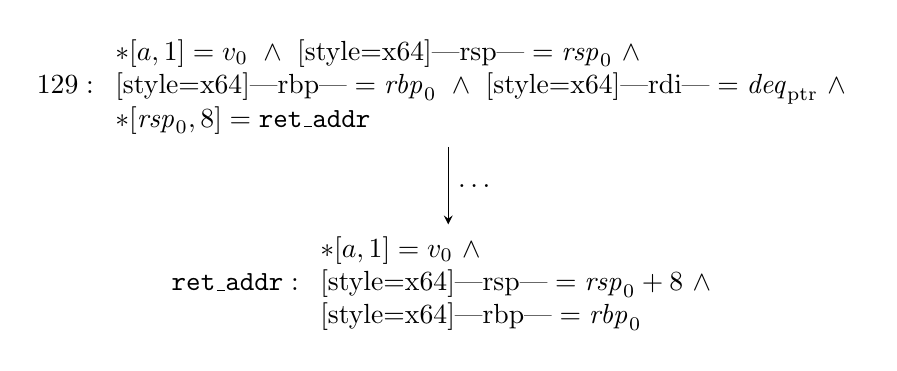
\begin{tikzpicture}[>={stealth}]
      \graph[math nodes, grow down=2.5cm]{
        a/"129:\begin{array}{l}
          \readmem{a}{1} = v_0~\wedge~\mathrsp = \rspo~\wedge \\
          \mathrbp = \rbpo~\wedge~\mathrdi = \deqptr~\wedge \\
          \readmem{\rspo}{8} = \retaddr
        \end{array}" ->[
          "\dots"
        ] b/"\retaddr:\begin{array}{l}
          \readmem{a}{1} = v_0~\wedge\\
          \mathrsp = \rspo + 8~\wedge\\
          \mathrbp = \rbpo
        \end{array}"
      };
    \end{tikzpicture}
    \caption{\lstinline|dequeue_push|}\label{fig:dequeue_push}
  \end{subfigure}
  \begin{subfigure}{.50\linewidth}
    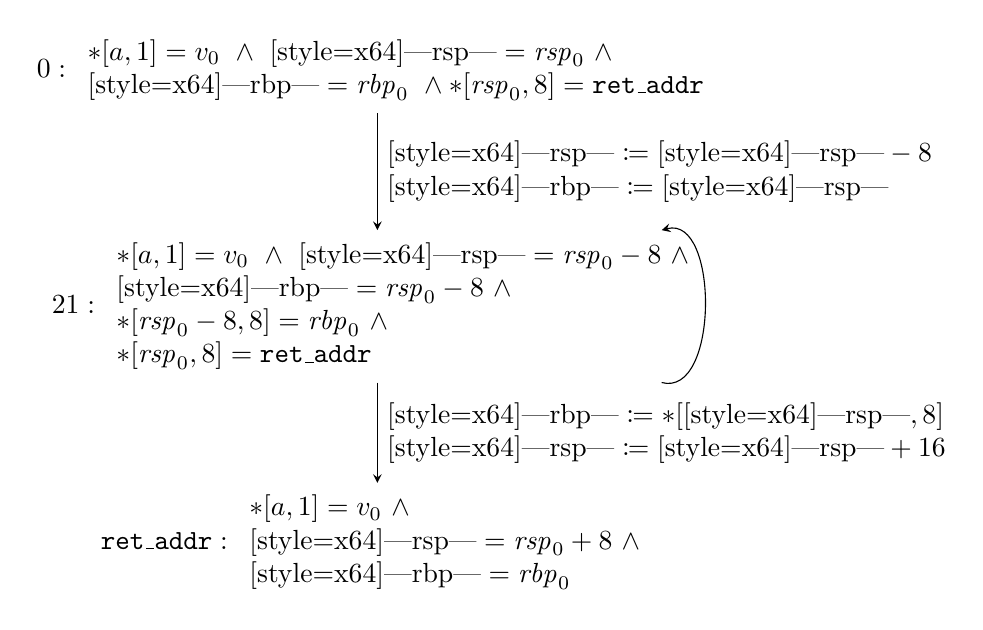
\begin{tikzpicture}[>={stealth}]
      \graph[math nodes, grow down=3cm]{
        a/"0:\begin{array}{l}
          \readmem{a}{1} = v_0~\wedge~\mathrsp = \rspo~\wedge \\
          \mathrbp = \rbpo~\wedge
          \readmem{\rspo}{8} = \retaddr
        \end{array}" ->[
          align=left,
          "$\mathrsp\coloneqq\mathrsp-8$\\
          $\mathrbp\coloneqq\mathrsp$"
        ] b/"21:\begin{array}{l}
          \readmem{a}{1} = v_0~\wedge~\mathrsp = \rspo-8~\wedge \\
          \mathrbp = \rspo-8~\wedge \\
          \readmem{\rspo-8}{8} = \rbpo~\wedge \\
          \readmem{\rspo}{8} = \retaddr
        \end{array}" ->[
          align=left,
          "$\mathrbp\coloneqq\readmem{\mathrsp}{8}$\\
          $\mathrsp\coloneqq\mathrsp+16$"
        ] c/"\retaddr:\begin{array}{l}
          \readmem{a}{1} = v_0~\wedge \\
          \mathrsp = \rspo + 8~\wedge \\
          \mathrbp = \rbpo
        \end{array}";
        b ->[out=-15, in=15, looseness=1] b;
      };
    \end{tikzpicture}
    \caption{\lstinline|buddy_large_avail|}\label{fig:buddy_large_avail}
  \end{subfigure}
  \caption{Example Floyd invariants}
\end{figure*}

\section{Limitations}
% TODO

  \chapter{Syntax-Driven Verification}\label{ch:syntax}
\acreset{fmuc} % just in case
While the methodology presented in the previous chapter
for verifying memory preservation works well, it is not ideal.
The need to manually formulate regions
and the amount of work required for developing invariants
reduces potential scalability.

In order to deal with those downsides,
this chapter introduces the concept of \acp{fmuc}
generated by untrusted, informal tools.
\Acp{fmuc} consist of two main components:
theorems on memory preservation and \emph{proof ingredients}.%
\index{proof!ingredient}
The proof ingredients are assumptions on memory layout,
control flow information, and invariants
generated to reduce the amount of work required from end users.

Certificate generation is presented in \cref{se:fmuc_gen},
while the process of verification in Isabelle is documented in \cref{se:fmuc_ver}.
A full example of \ac{fmuc} usage can then be found in \cref{se:syntax_example}.
That example could theoretically overwrite
its own return address due to its pointer arguments, causing \ac{cfi} issues.
The associated \ac{fmuc} provides preconditions to prevent such cases
along with a formal proof of return address preservation under those conditions.
Following the example in \cref{se:xen} is an in-depth case study
on the Xen Project hypervisor \autocite{chisnall2008definitive}.
In total, \acp{fmuc} were generated and proofs discharged in Isabelle
for 251 Xen functions.

My primary contributions to the certificate generation and verification approach%
\index{certificate}
presented in this chapter include the Hoare rules developed
for memory preservation as well as the \ac{vcg} used to apply those rules
to \ac{scf} in Isabelle (\cref{se:fmuc_ver}).
I also greatly expanded the code for full translation of the \acp{fmuc}
into the Isabelle/HOL language
and helped adapt the \ac{scf} into a form suitable for verification
in Isabelle (\cref{isabelle_scf}).
Additionally, I contributed to invariant generation (\cref{sse:inv_gen})
and performed much of the verification work for our large case study,
presented in \cref{se:xen}.

\section{\acs*{fmuc} Generation}\label{se:fmuc_gen}
\begin{figure*}
  \centering
  \begin{tikzpicture}[>=stealth, gnode/.style={draw, rounded corners, text centered}]
    \graph[grow right=2.8cm]{
      Assembly[gnode] ->[dashed]
      "Control Flow Graph"[gnode, text width=1.4cm] ->["\ref{sse:cfg_extract}"]
      "Syntactic Control Flow"[gnode, text width=1.7cm] ->["\ref{sse:syntax_symb}"]
      "Memory Regions and \acsp*{mrr}"[gnode, text width=1.5cm]
      ->["\ref{sse:inv_gen}"]
      Invariants[gnode] ->[dashed] Certificate[gnode];
    };
  \end{tikzpicture}
  \caption{Overview of \acs*{fmuc} generation}\label{fig:overview}
\end{figure*}

\Acp{fmuc} require the assembly code of a program as input.
That source assembly could be obtained from a binary using a disassembler, such as \texttt{objdump},
IDA\fturl{https://www.hex-rays.com/products/ida/index.shtml},
Ghidra's decompiler\fturl{https://ghidra-sre.org/}, or Capstone \autocite{capstone}.
If source code is available, it could be generated directly by a compiler instead.
Each function specified for verification receives \iac{fmuc};
those that are not included in the verification effort,%
\index{verification!effort}
including system calls and functions from dynamic libraries,
can be treated as black boxes,
the usage of which is described in \cref{sse:fmuc_comp}.

The general procedure for generating \acp{fmuc}, laid out in \cref{fig:overview},
can be broken up into three main parts.
The first part involves control flow extraction from the supplied assembly
using \iac{cfg} analysis similar to angr's CFGFast%
\index{angr!CFGFast}
\autocite{shoshitaishvili2016state},
ultimately producing \iac{scf} (the details of which are presented
in \cref{sse:cfg_extract}).
Afterwards, per-basic block symbolic execution
is utilized to generate the set of memory regions
read and written by the function in question.
This was detailed in \cref{ch:symbolic_execution}.
To eliminate duplicates and produce \acp{mrr}
showing which regions overlap or are enclosed or separate,
the region sets are then fed to the \ac{smt} solver Z3 \autocite{de2008z3}.
Symbolic execution is also used in the process of generating
the pre- and postconditions for each basic block,
elaborated on in \cref{sse:inv_gen}.

With the exception of \ac{mrr} generation,
none of the steps in this procedure are included in the \ac{tcb}.
The process of verifying the generated \ac{fmuc} (see \cref{se:fmuc_ver})
will fail if there are issues in control flow extraction,
\ac{scf} generation, informal symbolic execution, or invariant generation.
\Ac{mrr} generation is an exception
because the \acp{mrr} are formulated as assumptions,
and thus inconsistent \acp{mrr} will result in vacuous proofs.
This is why the methodology relies on Z3 for \ac{mrr} generation;
using a known-reliable tool greatly reduces the possibility of issues.

\subsection{Control Flow Extraction}\label{sse:cfg_extract}
As described in \cref{se:hoare},
in order to apply \iac{vcg} that utilizes Hoare rules to verify a Hoare triple,
there must be some syntactic structure to apply those rules to.
This chapter uses a syntactic representation of control flow called \ac{scf}
in part for that purpose.
\Ac{scf} expresses assembly programs as a combination of basic blocks,
branches, loops, and function calls.
The following grammar provides a description of \ac{scf}
produced by the extraction code.
Each basic block is represented by the polymorphic type~$\beta$,
while branching conditions are represented using the polymorphic type~$\Phi$.
\begin{bnf}
  \bnfprod*{scf}{
    \bnfpn{scf}\bnfsp\bnfts{;}\bnfsp\bnfpn{scf}
    \bnfor\bnfts{Block}\bnfsp\bnftd{$\beta$}
    \bnfor\bnfts{Skip}
    \bnfor\bnfts{Continue}
    \bnfor\bnfts{Break}\bnfsp\bnfpn{br}
  } \\
  \bnfmore{
    \bnfor\bnfts{If}\bnfsp\bnftd{$\Phi$}
      \bnfsp\bnfts{Then}\bnfsp\bnfpn{scf}
      \bnfsp\bnfts{Else}\bnfsp\bnfpn{scf}
      \bnfsp\bnfts{Fi}
    \bnfor\bnfts{Loop}\bnfsp\bnfpn{scf}\bnfsp\bnfts{Pool}\bnfsp\bnfpn{res}
  } \\
  \bnfprod{br}{
    \bnftd{ID}\bnfor\bnfes
  } \\
  \bnfprod{res}{
    \bnfts{Resume}\bnfsp\bnfts{\{(}\bnftd{ID}\bnfts{,}
      \bnfpn{scf}\bnfts{),}\bnfsk\bnfts{\}}
    \bnfor\bnfes
  }
\end{bnf}
Loops in this formulation have no exit condition;%
\index{loop}
instead, they rely on having one or more internal \texttt{Break} statements,%
\index{loop!break}
which may have an identifier to indicate how the loop was exited, for termination.
\texttt{Continue}s function the same as in C,%
\index{loop!continue}
causing loop execution to skip to the next iteration.
For loops that have multiple exit points,
\texttt{Resume} statements provide different code to execute
based on which exit was taken as indicated by the \texttt{Break} identifier.

Notably, the above data structure does not explicitly contain
control flow statements such as \texttt{goto} or \texttt{throw/catch}.
Unconditional jumps like \texttt{goto}s make code harder to reason about
in a structured way and can be modeled by the existing syntactic constructs,
while structured exception handling as used in \Cpp\ is generally provided
by external function calls%
\index{exception handling!functions}
(\cref{se:structured_exceptions}).
\begin{example}
  \Cref{fig:ex_cf} provides an example of \ac{scf} extracted from \iac{cfg}.
  The \ac{cfg} in \cref{fig:ex_cf_cfg} can be seen to have two branching conditions
  that do not involve loops, one from $\ABB~0$ with condition~$f_0$
  and one from $\ABB~7$ with condition~$f_7$.
  This leads to if statements with those conditions
  being added to the \ac{scf} in \cref{fig:ex_cf_scf} after their respective blocks.
  The one loop present has two exit points.
  If condition~$f_1$ is false after execution of $\ABB~1$,
  the loop will exit to $\ABB~4$, while $\ABB~2$ will exit to $\ABB~3$ if~$f_2$ is false.
  This leads to the $\ABreak$ statements present in the extracted \ac{scf}
  in their respective conditional statements
  annotated with the IDs for their associated exit blocks.
  Those two exit points also result in the generation of a $\AWhileResume$ clause
  indicating where those $\ABreak$s exit to.
  \begin{figure*}
    \hspace*\fill
    \subcaptionbox{Example \ac*{cfg}\label{fig:ex_cf_cfg}}{
      \begin{tikzpicture}[->, >=stealth, node distance=0.75cm]
        \node[draw=none] (0) {0};
        \node[draw=none] (1) [below=of 0] {1};
        \node[draw=none] (2) [below=of 1]{2};
        \node[draw=none] (3) [below=of 2]{3};
        \node[draw=none] (4) [left=of 3, xshift=0.5cm, yshift=0.5cm]{4};
        \node[draw=none] (5) [below=of 3]{5};
        \node[draw=none] (6) [below=of 5, xshift=0.5cm, yshift=0.5cm]{6};
        \node[draw=none] (7) [right=of 1]{7};
        \node[draw=none] (8) [right=of 3, xshift=0.5cm, yshift=0.5cm]{8};
        \node[draw=none] (9) [right=of 5]{9};

        \path (0) edge node[left]{$f_0$} (1);
        \draw[rounded corners=2mm] (0) -|
        node[above, xshift=0.4cm, yshift=-0.9cm]{$\neg f_0$} (7);
        \path (1) edge [bend left] node[right]{$f_1$} (2);
        \draw[rounded corners=2mm] (1) -| node[left, yshift=-1.3cm]{$\neg f_1$} (4);
        \path (2) edge [bend left] node[left, xshift=0.1cm]{$f_2$} (1);
        \path (2) edge node[right]{$\neg f_2$} (3);
        \path (3) edge node[right]{} (5);
        \draw[rounded corners=2mm] (4) |- (5);
        \path (5) edge node[right]{} (6);
        \draw[rounded corners=2mm] (7) -| node[right, yshift=-1.3cm]{$\neg f_7$} (8);
        \path (7) edge node[left, yshift=-1cm]{$f_7$} (9);
        \draw[rounded corners=2mm] (8) |- (9);
        \path (9) edge node[right]{} (6);
      \end{tikzpicture}
    }
    \hfill
    \subcaptionbox{Syntactic Control Flow\label{fig:ex_cf_scf}}{
      \(\begin{array}{l}
        \ABB~0\ASeq* \\
        \AIf~f_0~\AThen \\
        \ind{4ex}\AWhile \\
        \ind{8ex}\ABB~1\ASeq* \\
        \ind{8ex}\AIf~f_1~\AThen \\
        \ind{12ex}\ABB~2\ASeq* \\
        \ind{12ex}\AIf~f_2~\AThen~\AContinue~\AElse~\ABreak~2~\AFi \\
        \ind{8ex}\AElse \\
        \ind{12ex}\ABreak~1 \\
        \ind{8ex}\AFi \\
        \ind{4ex}\AOd~\AWhileResume~\{(2,\ABB~3),(1,\ABB~4)\}\ASeq* \\
        \ind{4ex}\ABB~5 \\
        \AElse \\
        \ind{4ex}\ABB~7\ASeq* \\
        \ind{4ex}\AIf~f_7~\AThen~\ASkip~\AElse~\ABB~8~\AFi\ASeq* \\
        \ind{4ex}\ABB~9 \\
        \AFi\ASeq* \\
        \ABB~6
      \end{array}\)
    }
    \hspace*\fill
    \caption{Example of control flow extraction}\label{fig:ex_cf}
  \end{figure*}
\end{example}

\subsubsection{Restrictions}
There two important restrictions on the current control flow extraction approach,
the more severe of which is the lack of support for indirect branching.
The \ac{cfg} analysis done by the current extraction algorithm
is not strong enough to handle indirect branching at the moment.
In some cases, the set of possible branches can be determined based on the
local function context, but the result of an indirect branch is often based off of input arguments, as well. Even if the result set
might be determinable with static analysis, it would have to be interprocedural,
and branch destinations based on external input cannot be determined.

Finally, as the if-then-else statement provides the sole form of
branching control flow, the algorithm is not optimal
due to the duplication of blocks to fit less structured control flow
into a more structured model. In the worst case,
it can result in \ac{scf} explosion, described below.

\subsubsection{\acs*{scf} Explosion}\label{sse:scf_explode}
The algorithm is not optimal in terms of generated \ac{scf} size
as certain basic blocks may be duplicated.
There are two situations where basic block duplication occurs,
one less common than the other.
The less common situation is when loop having multiple entry points,
which can occur in situations that involve less-structured control flow,
such as a C program that jumps into a loop using \texttt{goto}.
Such situations are relatively uncommon, even in optimized code.
If it does happen, the entire loop must be duplicated.
The more common situation, by contrast, involves complex conditional branching
that can occur even without loops.
\begin{example}
  \Cref{fig:ex_nonopt} shows a small example of branching control flow
  that results in $\ABB~3$ being duplicated.
  That block could itself be an even more complicated subgraph,
  possibly leading to exponential code duplication.
  \begin{figure*}
    \hspace*\fill
    \subcaptionbox{\acs*{cfg}}{
      \begin{tikzpicture}[>=stealth, ->, node distance=0.75cm]
        \node[draw=none] (0) {0};
        \node[draw=none] (1) [right=of 0] {1};
        \node[draw=none] (2) [right=of 1] {2};
        \node[draw=none] (3) [right=of 2] {3};
        \node[draw=none] (4) [right=of 3] {4};

        \path (0) edge node[below]{$f_0$} (1);
        \path (0) edge [bend left] node[above]{$\neg f_0$} (4);
        \path (1) edge node[above]{$f_1$} (2);
        \path (1) edge [bend right] node[below]{$\neg f_1$} (3);
        \path (2) edge node[above]{$f_2$} (3);
        \path (2) edge [bend right] node[below]{$\neg f_2$} (4);
        \path (3) edge (4);
      \end{tikzpicture}
    }
    \hfill
    \subcaptionbox{\acs*{scf}}{
      \(\begin{array}{l}
        \ABB~0; \\
        \AIf~f_0~\AThen~\ABB~1; \\
        \ind{4ex}\AIf~f_1~\AThen~\ABB~2; \\
        \ind{8ex}\AIf~f_2~\AThen~\ABB~3 \\
        \ind{8ex}\AElse~\ASkip~\AFi \\
        \ind{4ex}\AElse~\ABB~3~\AFi \\
        \AElse~\ASkip~\AFi; \\
        \ABB~4
      \end{array}\)
    }
    \hspace*\fill
    \caption{Example of code duplication}\label{fig:ex_nonopt}
  \end{figure*}
\end{example}

\subsection{Symbolic Execution for Generation}\label{sse:syntax_symb}
In \cref{sse:cfg_extract}, the semantics of assembly were expressed%
\index{semantics!assembly}
in terms of control flow between basic blocks.
This section now covers the symbolic execution of those individual blocks.
The Haskell symbolic execution engine
takes as input a data structure of type $\scf(B,E_F)$,
which is formulated over basic blocks,
and produces $\scf(\powerset(\gls{assign}),\gls{esp})$,
which is formulated over sets of assignments.
It keeps track of all used memory regions,
both the actual regions used by instructions as well as merged regions,
in order to supply those regions as part of an \ac{fmuc}.

\subsubsection{Generating Memory Region Relations}
Because symbolic execution uses symbolic state,
the relations of enclosure, separation, and overlap,
defined in \cref{memory_aliasing}, must be determined for symbolic expressions.
Unfortunately, there is no single solution, no one decision procedure,
that can determine these properties for all symbolic expressions automatically.

As an example of the potential issues that can occur,
take the completely symbolic regions $r_0=\region{a_0}{s_0}$
and $r_1=\region{a_1}{s_1}$.
Without additional information, we cannot determine any relations for these regions.
If they are \emph{possibly} different then they must be treated as different regions,
while if they \emph{necessarily} overlap
then they must be treated as a single merged region.

To deal with such symbolic issues,
the three aforementioned relations of enclosure, separation, and overlap
are formulated as \ac{smt} problems.
The \ac{smt} formulations are negations
of the equations presented in \cref{def:sep,def:enc};
the result states the property holds if the resultant problem is \emph{unsatisfiable}.
These \ac{smt} problems can be solved by Z3 \autocite{de2008z3}
for a wide range of expressions over bitvectors
using the \lstinline|QF_UFBV| logic \autocite{smtlib:bitvector-logic,smtlib:bitvector-theory}.
Z3 is also used in this work for determining the sign of two values
in the region merge algorithm, originally presented in \cref{def:merge}.
Additionally, reads of overlapping regions may require merging
and separation analysis as described in \cref{memory_aliasing},
so they also rely on Z3.

The result of evaluating the above \ac{smt} problems
over all pairs of memory regions for a basic block, each region being given a unique ID,
is two sets with element type $\gls{nat}\times\gls{nat}$, $\var{enc}$ and $\var{ovl}$.
Every element $(i_0,i_1)$ in $\var{enc}$ indicates that the region with ID~$i_0$
is enclosed by the region with ID~$i_1$.
Every element $(i_0,i_1)$ in $\var{ovl}$ indicates that the two regions with those IDs
overlap.
Those two sets are the \acp{mrr} for the block,
and using them as assumptions allows for efficient execution of the rewrite rules
in \cref{memory_rewrite}.

\subsection{Invariant Generation}\label{sse:inv_gen}
Invariants, formalized as sets of assignments of the aforementioned type~\gls{assign},
\index{invariant}
are generated by starting from a precondition for the entry point of the function
and \emph{propagating} it throughout.%
\index{invariant!propagation}

The initial precondition of the function as a whole is generated
by including initial symbolic values for all registers that are read
before they are written as well as all used memory regions
that are not enclosed in another.
The concrete initial value of the instruction pointer, \inlineasm{rip},
must also be included,
and the (symbolic) address to return to after function completion
must be indicated as stored on the stack.
In Haskell, the conditions in question are represented as sets of assignments.
\begin{example}[Initial invariant]
  To reuse \cref{ex:simple}, its initial precondition would be:
  \begin{equation}
    \phi=\{\mathrip\coloneqq\mathtt{a0},
    \mathrsp\coloneqq\rspo,
    \region{\mathrsp-8}{8}\coloneqq v_0,
    \region{\mathrsp}{8}\coloneqq\retaddr\}.
  \end{equation}%
  \nomenclature{$\phi$}{Denotes a generated invariant}
\end{example}
Propagation requires performing \emph{substitution},%
\index{invariant!substitution}
which is defined over assignments, state parts, and expressions,
all with respect to invariant~$\phi$.
\begin{subequations}
  \begin{align}
    \subst(\phi,\var{sp}\coloneqq v) &= \subst(\phi,\var{sp})\coloneqq\subst(\phi,v)\\
    \subst(\phi,\var{sp}) &= \text{if }\exists v\cdot(\var{sp},v)\in\phi
    \text{ then }v\text{ else }\var{sp} \\
    \subst(\phi,e_0\bop e_1) &= \text{if }\exists v\cdot(e_0\bop e_1,v)\in\phi
    \text{ then }v\text{ else }\subst(\phi,e_0)\bop\subst(\phi,e_1) \\
    \text{unary ops} &= \dotso \notag \\
    \text{ternary ops} &= \dotso \notag
  \end{align}
\end{subequations}%
\nomenclature[operator]{$\bop$}{Denotes an arbitrary binary operator}

\Cref{algo:prop} performs invariant propagation.
Each block is modified by applying all applicable substitutions
with respect to~$\phi$.
Invariant~$\phi$ is then modified based off of the semantics of the block.%
\index{semantics}
Treating~$\alpha$ as the set of assignments in the block,
$\phi$ is modified by taking the subset of substitutions
where the substitutees are overwritten by~$\alpha$
and combining them with the subset of substitutions
that were completely unmodified by any assignment in~$\alpha$:
\begin{equation}
  \post(\phi,\alpha)\footnote{%
    This is a different $\post$ from that used to identify \ac{cfg} block children.
  }\equiv\{(v,e)\mid(v\coloneqq e\in\alpha\land(v,\_)\in\phi)
  \lor((v,e)\in\phi\land(v,e)\text{ is unmodified by }\alpha)\}.
\end{equation}
\begin{example}[Invariant propagation]
  Once again consider \cref{ex:simple}.
  Propagation of the initial precondition through the single basic block
  produces the following postcondition:
  \begin{equation}
    \begin{split}
      \phi=\{\mathrip &\coloneqq\retaddr, \\
      \mathrsp &\coloneqq\rspo+8, \\
      \region{\rspo-8}8 &\coloneqq\mathtt{0xAABBCCDD}\concat
      \takebits{31,16}v_0\concat\mathtt{0xEEFF}, \\
      \region{\rspo}8 &\coloneqq\retaddr\}.
    \end{split}
  \end{equation}
\end{example}
\begin{algorithm}
  \caption{Invariant propagation}\label{algo:prop}
  \begin{algorithmic}
    \Require{Input is of type $\scf(\powerset(\gls{assign}),\gls{esp})$}
    \Ensure{Output is a tuple of possibly-updated~$\phi$
      and \ac{scf} updated with current~$\phi$:
      $\gls{assign}\times\scf(\powerset(\gls{assign}),\gls{esp})$}
    \Function{prop}{$\phi,\ABB~\alpha$}
      \State $\phi'\gets\post(\phi,\subst(\phi,\alpha))$
      \State\Return $(\phi',\ABB~(\alpha\text{ annotated with }\phi))$
    \EndFunction
    \Function{prop}{$\phi,\alpha_0\ASeq \alpha_1$}
      \State $(\phi',\alpha_0')\gets\Call{prop}{\phi,\alpha_0}$
      \State $(\phi'',\alpha_1')\gets\Call{prop}{\phi',\alpha_1}$
      \State\Return $(\phi'',\alpha_0'\ASeq \alpha_1')$
    \EndFunction
    \Function{prop}{$\phi,\AIf~f~\AThen~\alpha_0~\AElse~\alpha_1~\AFi$}
      \State $(\phi_0,\alpha'_0)\gets\Call{prop}{\phi,\alpha_0}$
      \State $(\phi_1,\alpha'_1)\gets\Call{prop}{\phi,\alpha_1}$
      \State $\phi'\gets\phi_0\cap\phi_1$
      \State\Return $(\phi',\AIf~\subst(\phi,f)~\AThen~
        \alpha'_0~\AElse~\alpha'_1~\AFi)$
    \EndFunction
    \Function{prop}{$\phi,\AWhile~\alpha~\AOd$}
      \State $(\phi',\alpha')\gets\Call{prop}{\phi,\alpha}$
      \If{$\phi\subseteq\phi'$}%
        \nomenclature[operator]{$\subseteq$}{Indicates subset relation}
        \State\Return $(\phi,\AWhile~\alpha'~\AOd)$
      \Else
        \State\Return $\Call{prop}{\phi\cap\phi',\AWhile~\alpha~\AOd}$
      \EndIf
    \EndFunction
    \Function{prop}{$\phi,\AWhileResume~\var{resumes}$}
      \ForAll{$\alpha_i\in\var{resumes}$}
        \State $(\phi'_i,\alpha'_i)\gets\Call{prop}{\phi,\alpha_i}$
      \EndFor
      \State $\phi''\gets\bigcap\phi'$
      \State\Return $(\phi'',\AWhileResume~\Call{zip}{i,\alpha'})$
    \EndFunction
    \Function{prop}{$\phi,\alpha$}\Comment{Default case}
      \State\Return $(\phi,\alpha)$
    \EndFunction
  \end{algorithmic}
\end{algorithm}
Invariant propagation is straightforward for sequencing and if statements,
with sequencing simply chaining invariant propagation
and if statements producing an invariant that is the common result
of propagating the initial invariant down both branches.

In contrast, a loop with body~$\alpha$ requires continual propagation
until the invariant~$\phi$ stabilizes, possibly by becoming~$\varnothing$.%
\nomenclature{$\varnothing$}{The empty set}
This stabilization is identified
by checking if~$\phi$ is a subset of its propagated self.
If it is, then \textsc{prop} returns the propagated~$\phi$
and a new loop with the propagated body.
Otherwise,
the original loop is propagated again with the intersection of~$\phi$
and its propagated self.
This process effectively computes the loop invariant
as the greatest subset of the initial invariant
that is preserved by execution of the loop body.
For loops that have multiple exits,
each exit's resume is propagated with the invariant at the point of exit evaluation.
In a similar fashion to the process for if statements,
the invariants that result from individual resume propagation
are intersected to produce a singular invariant for all resumes,
which is then returned along with all of the propagated resumes.

\section{\acs*{fmuc} Verification}\label{se:fmuc_ver}
This section presents verification of \iac{fmuc} as shown in \cref{fig:verify},
one of the primary contributions for this chapter as mentioned in its preamble.
Both the \ac{fmuc} and the original assembly are loaded into Isabelle/HOL,
where the memory preservation theorem is then proven using the proof ingredients
provided by the \ac{fmuc}.
By this method, which requires a step function
that models the semantics of the assembly instructions
and a process to apply it repeatedly,
the \ac{fmuc}'s memory preservation Hoare triple can be verified.

\begin{figure*}
  \centering
  \begin{tikzpicture}[->, >=stealth, every node/.style={
    draw,
    rounded corners,
    text width=3cm,
    text centered,
    minimum height=1.5cm
  }]
    \node (a) {Isabelle/HOL};
    \node[above left=of a] (b) {Assembly};
    \node[below left=of a] (c) {Certificate};
    \node[right=1.5cm of a] (d) {OK/unproven};

    \draw (b) -- (a.north west);
    \draw (c) -- (a.south west);
    \draw (a) -- (d);
  \end{tikzpicture}
  \caption{Overview of \acs*{fmuc} verification}\label{fig:verify}
\end{figure*}

\subsection{Syntactic Control Flow in Isabelle/HOL}\label{isabelle_scf}
As described previously, \acl{scf} is a representation of the control flow of a function
in terms of syntactic structures such as basic blocks,
loops, and if-then-else statements.
While very similar to the \ac{scf} used when generating \acp{fmuc},
there are some modifications that must be made when the generated \acp{scf}
are to be loaded into Isabelle/HOL.
These modifications are required due to subtle differences in the semantics
of the generating tool versus the verifying tool,
and are required to properly support the Hoare rules
described in \cref{scf_hoare} below.

In the Isabelle/HOL representation,
there are no \texttt{Break}s or \texttt{Continue}s;
any occurrences of such statements are translated to \texttt{Skip}.
This does mean that programs that cannot be easily transformed
such that that translation does not modify the overall semantics
are not easily handled in this framework.
However, none of functions encountered in the case study presented in \cref{se:xen}
had that issue, so it does not appear to be a significant drawback.

Additionally, loops in the Isabelle/HOL \ac{scf} syntax
do rely on a explicit exit condition.
This condition is simply the precondition of the entry block of the loop
as generated using the methodology in \cref{sse:inv_gen}.

Another important difference is that basic blocks in Isabelle
take the form $\ABB~\Block*{n}{a}{i}$,
where~$n$ indicates the number of instructions in the block,~$a$ is the address
of the last instruction in the block, and~$i$ is an ID
that uniquely identifies the block in the current \ac{scf}.
This style is used to assist with the symbolic execution methodology described in
\cref{sse:syntax_ver_symb}.

Finally, to properly handle function calls in the Isabelle/HOL syntax,
the analyzed \acp{cfg} are preprocessed prior to performing extraction
in order to isolate \inlineasm{call} instructions into their own basic blocks.
% Freek did the preprocessing but I did all the rest.
These single-instruction blocks are then translated into \texttt{Call}~$f$ entries
in the Isabelle/HOL \ac{scf}, where~$f$ is the textual label of the function called.
This allows for proper matching with the Hoare rules presented below.

\subsection{Symbolic Execution for Verification}\label{sse:syntax_ver_symb}
\Cref{cfg_symb_exec} previously presented a formal symbolic execution engine
based on the machine model described in \cref{se:machine_model}.
It provides a function $\run$ that describes the symbolic execution of
blocks in a control flow graph.

The formal function for block-level symbolic execution presented in this chapter,%
\index{symbolic!execution}
by contrast, is a \emph{transition relation}%
\index{transition relation} formulated as
\begin{equation*}
  \execblock:\gls{nat}\times W\times\gls{nat}\times S\times S\rightarrow\gls{bool}.
\end{equation*}
Its inputs are the number of instructions left to execute in the block,
the address of the last instruction in the block, the block's ID,
the current state~$\sigma$, and an ending state~$\sigma'$.
Its result is true if and only if execution
starting from the current instruction in state~$\sigma$
and running to the ending address can produce state~$\sigma'$.
The other arguments are used to ensure termination and block matching.
Undefined behavior, such as null-pointer dereferencing,
is modeled by relating the state in which it occurs to any successor state
supplied with it.

The internal step function has type $\gls{step}:A\times\gls{nat}\times S\rightarrow S$,
with its first argument being an instruction, its second being the size of the instruction,
and its third being the current state.
The function returns the state after instruction execution,
incrementing \inlineasm{rip} by the supplied size
if it was not changed by a control-flow instruction instead.

% TODO: provide the detail of the $\exec$ function if time permits
The $\execblock$ function is used internally by another transition relation,
this one for the symbolic execution of entire \acp{scf}:
$\exec:\var{SCF}\times S\times S\rightarrow\mathbb{B}$.
That function recurses through \iac{scf}
and checks $\execblock$ on every block it finds,
performing the necessary state transformations to deal with the semantics of
the individual \ac{scf} components encountered.
Any loops encountered are dealt with using \iac{lfp} construction.
This means that, if there are any infinite loops present,
the function will have no related successor states.
The only matching state would be $\infloop$.
Strictly speaking, $\exec$ is not actually executed when used in \ac{fmuc} proofs;
it exists to allow proving the correctness
of the Hoare rules shown below in \cref{scf_hoare}.

Unlike the symbolic execution for generation,
this symbolic execution methodology is implemented fully in Isabelle/HOL,
meaning that every rewrite rule has been formally proven correct.

\subsection{Per-Block Verification}\label{sse:per-block}
The verification methodology presented here occurs
by first verifying the functionality of each basic block in the corresponding function.
This is done for each block by proving the lemma shown below,
using the $\exec$ function from the previous section.
To do this, however, a formal notion of \emph{memory preservation}
with respect to state changes is required.
\begin{definition}[Memory preservation with respect to state changes]\label{def:mem_preserve}
  The set of memory regions~$M'$ characterizes memory preservation with respect to
  the change from some state~$\sigma$ to some other state~$\sigma'$
  if and only if every byte outside of the regions in~$M'$ is the same in both states.
  The addresses of those bytes are represented by the variable~$a$.

  This is formally expressed as:
  \begin{equation}
    \usage(M',\sigma,\sigma')\equiv\forall a\cdot(\forall r\in M'\cdot\region{a}1\gls{separate}r)
    \longrightarrow\readmemS{\sigma}a{1}=\readmemS{\sigma'}a{1}.
  \end{equation}
\end{definition}

Using \cref{def:mem_preserve}, each block gets a lemma of the form
\begin{equation}
  P(\sigma)\longrightarrow\execblock(n,a,i,\sigma,\sigma')\land
  Q(\sigma')\land\usage(M(\sigma),\sigma,\sigma').\label{eq:block_lemma}
\end{equation}
Note that~$M$ is a state-dependent function.
Every generated version of \cref{eq:block_lemma} is discharged
with an Isabelle/HOL proof method written in Eisbach \autocite{matichuk2016eisbach},
Isabelle's proof automation language.
For each block, the method takes the block-related proof ingredients
from the \ac{fmuc} and runs symbolic execution
to prove the postcondition and thus establish memory preservation for the block.
The open variables $P$, $Q$, $n$, $a$, $i$, and $M$ are all provided by the \ac{fmuc}.
No user interaction is required outside of cases where semantics
for specific instructions are unavailable or the Isabelle libraries in use
do not have the right simplification lemmas for automatic reasoning.
Those cases are rare and become rarer as more relevant lemmas are developed,
so for basic blocks, the proof is essentially automated.

\subsection{Function Body Verification}
While symbolic execution works well to establish memory preservation on the level of basic blocks,
the goal of this verification effort is to formally establish memory preservation
on the function level. This section describes that process,
which occurs after the individual blocks have had their semantics and memory preservation derived
and relies on Hoare logic (described in \cref{se:hoare}).

\subsubsection{Hoare Rules}\label{scf_hoare}
The Hoare triple formulation used for this work, $\htriple*{P}f{Q}M$,
resembles traditional Hoare triples a bit more than the version from \cref{ch:cfg},%
\index{Hoare!triple}
as rather than a halting condition
it takes a syntactic representation of the program, an \ac{scf}.
Unlike traditional Hoare triples, however,
it also explicitly contains the set of memory regions,~$M$,
that contain the areas of memory read and written by the program the \ac{scf} encodes.
Syntactic structure is required because Hoare logic is a syntax-guided approach.
\begin{definition}[Hoare triple for \ac{scf}]\label{def:preserve}
  \begin{equation}
    \htriple*{P}f{Q}{M}\equiv
    \forall\sigma~\sigma'\cdot P(\sigma)\land\exec(f,\sigma,\sigma')\longrightarrow
    Q(\sigma')\land\usage(M,\sigma,\sigma')
  \end{equation}
\end{definition}
The above definition states the following:
if precondition~$P$ holds on the initial state~$\sigma$
and~$\sigma'$ would be the result of symbolically executing the \ac{scf}~$f$,
postcondition~$Q$ will hold on the produced state
and any values stored in the regions of memory outside set~$M$ remain unchanged.

While \cref{def:preserve} focuses on the regions written to,
the regions read must also be included as symbolic execution
relies on those regions being included.
Without them, proofs that require symbolically executing
the related instructions will not complete.
\begin{figure*}
  \centering
  \setlength\parskip{1em}
  \subcaptionbox{Introduction rule\label{fig:intro-rule}}{
    \AxiomC{$\begin{multlined}
      \forall\sigma~\sigma'\cdot P(\sigma)\longrightarrow \\
      \execblock(n,a,i,\sigma,\sigma')\land{} \\
      Q(\sigma')\land\usage(M(\sigma),\sigma,\sigma')
    \end{multlined}$}
    \AxiomC{$M'=\{r\mid\exists\sigma\cdot P(\sigma)\land r\in M(\sigma)\}$}
    \BinaryInfC{$\htriple*{P}{\ABB~\Block*{n}{a}{i}}{Q}{M'}$}
    \DisplayProof
  }

  \subcaptionbox{Sequence rule}{
    \AxiomC{$\htriple*{P}f{Q}{M_1}$}
    \AxiomC{$\htriple*{Q}g{R}{M_2}$}
    \AxiomC{$M=M_1\cup M_2$}
    \TrinaryInfC{$\htriple*{P}{f\ASeq g}{R}{M}$}
    \DisplayProof
  }

  \subcaptionbox{Conditional rule}{
    \AxiomC{$\htriple*{P\land B}f{Q_1}{M_1}$}
    \AxiomC{$\htriple*{P\land\neg B}g{Q_2}{M_2}$}
    \AxiomC{$Q_1\lor Q_2\longrightarrow Q$}
    \AxiomC{$M=M_1\cup M_2$}
    \QuaternaryInfC{$\htriple*{P}{\AIf~B~\AThen~f~\AElse~g~\AFi}{Q}{M}$}
    \DisplayProof
  }

  \subcaptionbox{While rule\label{fig:hoare-loop}}{
    \AxiomC{$\htriple*{I\land B}f{I'}{M}$}
    \AxiomC{$I'\longrightarrow I$}
    \AxiomC{$I\land\neg b\longrightarrow Q$}
    \TrinaryInfC{$\htriple*{I}{\texttt{While}~B\texttt{ DO }f\texttt{ OD}}{Q}{M}$}
    \DisplayProof
  }
  \hfill
  \subcaptionbox{Skip rule}{
    \AxiomC{$M=\varnothing$}
    \AxiomC{$P\longrightarrow Q$}
    \BinaryInfC{$\htriple*{P}\ASkip{Q}{M}$}
    \DisplayProof
  }\hspace*\fill

  \subcaptionbox{Resume rule}{
    \AxiomC{$\forall {0\leq j\leq n}\cdot\htriple*{P}{a_j}{Q_j}{M_j}$}
    \AxiomC{$(\bigvee_{0\leq j\leq n} Q_j)\longrightarrow Q$}
    \AxiomC{$M = \bigcup_{0\leq j\leq n}M_j$}%
    \nomenclature[operator]{$\bigcup$}{Repeated union over a sequence or set of sets, akin to sum/product notation}
    \TrinaryInfC{$\htriple*{P}{\AWhileResume\{(i_0,a_0),\dotsc,(i_n, a_n)\}}{Q}{M}$}
    \DisplayProof
  }

  \hspace*\fill
  \subcaptionbox{Precondition weakening\label{fig:hoare-weaken}}{
    \AxiomC{$P\longrightarrow P'$}
    \AxiomC{$\htriple{P'}b{Q}{M}$}
    \BinaryInfC{$\htriple{P}b{Q}{M}$}
    \DisplayProof
  }
  \hfill
  \subcaptionbox{Postcondition strengthening}{
    \AxiomC{$Q'\longrightarrow Q$}
    \AxiomC{$\htriple*{P}b{Q'}{M}$}
    \BinaryInfC{$\htriple*{P}b{Q}{M}$}
    \DisplayProof
  }\hspace*\fill
  \caption{Hoare rules for memory preservation}\label{fig:rules}
\end{figure*}
\subsubsection{The Introduction Rule}
This rule, depicted in \cref{fig:intro-rule},
is the rule that ties the per-block verification to the function-body verification.
The first assumption requires the symbolic execution method be run
from a universally quantified initial symbolic state~$\sigma$ that satisfies the precondition.
As long as any resulting state~$\sigma'$ satisfies the postcondition~$Q$,
the set of memory regions~$M$ generated for the block should be correct.

The second assumption is required because of an important subtlety:
the regions generated in the~\ac{fmuc} are state dependent.
As previously stated,
the~$M$ for a block is actually a function based on the block's initial state:
its regions depend on the values stored in memory.
However, it makes no sense to express the regions used by individual blocks
within a larger function in terms of their own individual initial state alone.
It would be unsound for regions that depend on values calculated
in the middle of the function to be expressed solely in terms of the initial state.
As such,
the Hoare triples are defined over a state-independent set of memory regions,~$M'$.
That set is obtained for each block
by taking the generated state-dependent set of memory regions
and applying that set to any state that satisfies the current invariant.

\subsubsection{The Other Rules}
While the introduction rule for basic blocks
is the ultimate target of our Hoare rule application process,
the rest of the rules are required to decompose the syntax above the level of blocks.
The remainder of \cref{fig:rules} describes those additional rules.
The Sequence, Conditional, and Resume rules are straightforward:
their ultimate memory region sets are the unions of the region sets of their constituents.
Note that the sequence rule is sound only because the memory predicates
are independent of state as discussed in \cref{sse:per-block}.

The while rule is based on a loop invariant,~$I$.
If the memory preservation of one iteration of loop body~$f$
is constrained to set of memory regions~$M$,
then so is the memory preservation of every other iteration.
This may sound counterintuitive,
so consider a simple C-like loop that starts from $i=0$ and iterates while $i<10$.
The body of this example loop contains single-byte array assignment operations
along the lines of $a[i]=v$.
Verification of the loop requires the loop invariant $I(\sigma)=i(\sigma)<10$.
The \ac{fmuc} of the loop body will have, as a state-dependent set of memory regions, $M(\sigma)=\{\region{a+i(\sigma)}1\}$, which is a single region of one byte.
If the Hoare logic introduction rule were to be applied to the block
that is the body of the loop, the result would be as follows:
\begin{subequations}
  \begin{align}
    M' &= \{r\mid\exists\sigma\cdot I(\sigma)\land r\in M(\sigma)\} \\
    &= \{r\mid\exists\sigma\cdot i(\sigma)<10\land r=\region{a+i(\sigma)}1\} \\
    &= \{\region{a'}1\mid a\leq a'\le a+10\}
  \end{align}
\end{subequations}
The set~$M'$ contains the regions of memory used by the entire loop,
not just one iteration.
This is because the introduction rule applies the state-dependent set of memory regions
to any state that satisfies the invariant.
Thus, the strength of the generated invariants directly influences
the tightness of the overapproximation of memory preservation
and of memory usage as a whole.
A weaker invariant, such as $i<20$, would result in a larger set of memory regions
by relaxing the constraints on symbolic addresses and,
for other situations, symbolic region sizes.

\subsubsection{Verification Condition Generation}\label{sse:vcg}
\begin{lstlisting}[
  gobble=2,
  float=*,
  caption=VCG step method,
  label=lst:vcg_step,
  escapechar=|
]
  method vcg_step =
    ((rule htriples)+, rule blocks)+,
    (simp add: pred_logic Ps Qs)?, |\label{step_simp}|
    (((auto simp: eq_def)[])+)? |\label{step_auto}|
\end{lstlisting}
\begin{lstlisting}[gobble=2, float=*, caption=Main VCG method, label=lst:vcg]
  method vcg uses scf =
    subst scf,
    vcg_step+
\end{lstlisting}
The \ac{vcg} presented here is a set of Eisbach proof methods,
the entry point of which is shown in \cref{lst:vcg}.
It is designed to automatically apply the proper Hoare logic rules
as much as possible via the \lstinline|vcg_step| method in \cref{lst:vcg_step},
driven by the formal \ac{scf} provided by the \ac{fmuc}.

Internally, \lstinline|vcg_step| repeatedly applies one of the Hoare rules
from \cref{fig:rules} (excluding the While, strengthening, and weakening rules)
to the current state of the \ac{scf} until no more rules can be applied.
At that point, it assumes that the introduction rule has been applied,
resulting in a block goal being generated, and attempts to discharge that goal
using one of the lemmas generated for \cref{sse:per-block}.
This process is repeated until no more of the restricted set of rules can be applied
or the last rule application resulted in a non-block goal.
At that point, \cref{step_simp} cleans up any preconditions and postconditions
in the current goal.
The last step, \cref{step_auto}, then tries to eliminate as many goals as it can,
one at a time, with Isabelle's basic \lstinline|auto| method.
If there are no loops present in the \ac{scf} under consideration,
this method will complete the proof without any need for user interaction.

\begin{lstlisting}[
  gobble=2,
  float=*,
  caption=Alternate step method for $\AWhileResume$ clauses,
  label=lst:vcg_cases,
  escapechar=|
]
  method vcg_step' =
    (rule htriples)+,
    simp,
    ((rule htriples)+, rule blocks)+,
    (simp add: pred_logic Ps Qs)?,
    (((auto simp: eq_def)[])+)?
\end{lstlisting}
\begin{lstlisting}[
  gobble=2,
  float=*,
  caption=VCG method for loops,
  label=lst:vcg_while,
  escapechar=*
]
  method vcg_while for P :: state_pred =
    ((rule htriples)+)?,
    rule HTriple_weaken[where P=P], *\label{step_weaken}*
    simp add: pred_logic Ps Qs,
    rule HTriple_while,
    vcg_step+,
    (simp add: pred_logic Ps Qs)+,
    (
      (vcg_step' | vcg_step)+,
      (simp+)?
    )?
\end{lstlisting}
In the case where loops are present,
the \ac{vcg} provides an alternate \lstinline|vcg_while| method,
shown in \cref{lst:vcg_while}
that relies on the loop rule presented in \cref{fig:hoare-loop}.
That loop rule is structured such that
the majority of work required to support the loops
is identifying the preconditions of their exit blocks
and then supplying their disjunction to \lstinline|vcg_while|.
This method relies on application of the weakening rule
presented in \cref{fig:hoare-weaken} on \cref{step_weaken}
to show that the postcondition of the block before entry implies the loop invariant.

The method \lstinline|vcg_step'|, used within \lstinline|vcg_while|,
is provided for those cases where a loop has multiple exit points.
A $\AWhileResume$ statement will be present in such cases,
and the process of rule application and simplification must occur
in a slightly different order. On occasion, there will also be a loop that has a single
exit point but gets a $\AWhileResume$ statement anyway
due to how the control flow extraction algorithm is set up.
The process of dealing with such statements is roughly the same, however.

After application of \lstinline|vcg_while|,
nested loops and those with multiple exit points may require
additional applications of condition simplifying or plain \lstinline|simp| usage
around further applications of \lstinline|vcg_step|.
Nothing beyond that should be necessary.

Without exception, each of the proofs we produced
could be finished using standard, off-the-shelf Isabelle/HOL methods,
though finishing them was not always an automatic process.
The part that is usually the most involved,
defining the invariants (as seen in the previous chapter)
is taken care of by the \ac{fmuc} generation.
This leaves dealing with loops, particularly ones with multiple exit points,
as the biggest challenge for most situations.

\subsection{Composition}\label{sse:fmuc_comp}
In order to achieve a scalable verification methodology,
it must support some form of compositionality.

Consider the body of an already-verified function~$f$
with the following Hoare triple:
\begin{equation*}
  \htriple*{P_f}f{Q_f}{M_f}.
\end{equation*}
In order to reuse that function's proof in a compositional fashion,%
\index{function!composition}
it is treated as a black box.%
\index{function!black box}
Now consider the assembly of a function~$g$ that calls~$f$:
\begin{lstlisting}[style=x64, gobble=2, numbers=none]
  a0: push rbp
  a1: call f
  a2: pop  rbp
  a3: ret
\end{lstlisting}
$P$ and~$Q$ are the pre- and postconditions just before executing \inlineasm{call}
and just after it returns.
$P$ contains the equality $\readmem{\rspo^g-8}{8}=\rbpo^g$,
expressing that~$g$ has pushed the frame pointer \inlineasm{rbp}%
\index{frame!pointer}
into its own local stack frame.%
\index{stack!frame}
The ultimate postcondition of~$g$
expresses that the callee-saved register \inlineasm{rbp} is properly restored:%
\index{register!callee-saved}
$\mathrbp=\rbpo^g$.
That operation is indeed performed by \inlineasm{pop rbp}.
In order to prove proper restoration of \inlineasm{rbp},
a proof that function~$f$ did not overwrite any byte in the region%
\index{memory!region}
$\region{\rspo^g-8}{8}$ is required.
The proof must also show that~$f$ does not overwrite region $\region{\rspo^g}{8}$,
which stores the address~$g$ returns to.
That proof would be specific to this particular instance of calling~$f$.

Of course,~$g$ may not be the only function that calls~$f$.
It may even be called multiple times by the same function.
Every call has specific requirements on which memory regions must be preserved,
based on the calling context.
Thus, to be able to verify function~$f$ once
but reuse its proof for each call,
the proof must at least contain an overapproximation
of the memory written to by function~$f$.
This is exactly what \emph{separation
logic} \autocite{o2001local,reynolds2002separation,krebbers2017essence}%
\index{separation logic}
requires.
As described in \cref{sse:composition},
separation logic provides a \emph{frame rule} for compositional reasoning.%
\index{separation logic!frame rule}
Informally, this rule states that, if a program can be confined
to a certain part of state, properties of that program will carry over
when the program is used as part of a bigger system.

In order to achieve that same behavior specifically for memory preservation verification,%
\index{memory!preservation}
we developed the frame rule presented in \cref{fig:composition}.
This rule is used to prove that the memory usage of a caller function~$g$
is equal to the memory it itself uses, \emph{plus} the memory used by function~$f$.
It must have the following four assumptions.
First, that~$f$ has been verified for memory preservation,
with~$M_f$ denoting the memory regions~$f$ uses.%
\index{memory!region}
Second, that precondition~$P$ can be split up into two parts:
precondition~$P_f$, required to verify~$f$, and a separate part~$\psep$.
The separate part is specific to the specific call of the function
where the frame rule is applied.%
\index{separation logic!frame rule}
In the example above,~$P_\mathrm{sep}$ must contain the equality
$\region{\rspo^g-8}{8}=\rbpo^g$.
Third, the correctness of~$M_f$, the set of memory regions,
should suffice to prove that~$\psep$ is preserved.
This effectively means that, for the above example,~$M_f$
should not overlap with the two regions of~$g$.
Fourth and finally,~$\psep$ and~$Q_f$ should imply postcondition$~Q$.
\begin{figure*}
  \begin{prooftree}
    \def\defaultHypSeparation{\hskip.18in}
    \AxiomC{$\htriple*{P_f}{f}{Q_f}{M_f}$}
    \AxiomC{$P\longrightarrow P_f\land\psep$}
    \AxiomC{$\forall s~s'\cdot\begin{array}{l}
      (\usage(M_f,s,s')\land{} \\
      \psep(s))\longrightarrow\psep(s')
    \end{array}$}
    \AxiomC{$Q_f\land\psep\longrightarrow Q$}
    \QuaternaryInfC{$\htriple*{P}{\ACall f}{Q}{M_f}$}
  \end{prooftree}
  \caption{Frame rule for composition of memory usage}\label{fig:composition}
\end{figure*}

In practice, many functions will not be part of the assembly code under verification, such as dynamic library or system calls.
Those cases necessitate generating the assumptions required
to proceed with verification.
The following box notation supports those cases:
\begin{equation}
  \htriple*P{\fbox f}Q{M_f}\equiv
  \exists P_f~Q_f~\psep\cdot
  \text{all four assumptions of the frame rule are satisfied}.
\end{equation}
This assumption informally expresses that function~$f$ has been verified.
Its memory usage~$M_f$ is assumed to suffice to prove that
the states that satisfy precondition~$P$ lead to the states that satisfy
postcondition~$Q$.

\section{Full Example}\label{se:syntax_example}
This section presents an execution of the entire toolchain
on the example given in \cref{fig:example2-c}
as a summary of \cref{se:fmuc_gen,se:fmuc_ver}.
The~C code is provided solely for presentation,
as the only inputs to the \ac{fmuc} generation
are the assembly created by disassembling the corresponding binary%
\index{assembly}%
\index{assembly!dis-}%
\index{binary}
and a basic configuration file indicating which functions to analyze.
\Cref{fig:example2-scf} presents the generated \ac{scf}.
The example has one loop, which starts at instruction address \texttt{0x120}.%
\index{loop}
\begin{figure}
  \begin{subfigure}[b]{.53\linewidth}
    \begin{lstlisting}[language=C, gobble=6]
      int main(int argc, char* argv[]) {
          int* a = (int*)argv;
          int* b = (int*)(argv + 4);
          *(int*)(argv + 2) = *a + *b;
          *(char*)argv = 'a';

          int array[argc];
          for (int i = 0; i < argc; i++)
              array[i] = argv[i][0] * 2;

          if (is_even(argc))
              return array[argc];
          return array[0];
      }
    \end{lstlisting}
    \caption{C code}\label{fig:example2-c}
  \end{subfigure}%
  \hfill
  \begin{subfigure}[b]{.46\linewidth}
    \begin{equation*}
      \begin{array}{l}
        \ABB~\Block{1149}{120b}\ASeq* \\
        \AWhile \\
        \ind{2ex}\ABB~\Block{123e}{1244}\ASeq* \\
        \ind{2ex}\AIf~\var{SF}\neq\var{OF}~\AThen~\ABB~\Block{120d}{123a} \\
        \ind{4ex}\AElse~\ABreak~\AFi \\
        \AOd\ASeq* \\
        \ABB~\Block{1246}{1249}\ASeq* \\
        \ABB~\Block{124b}{124b}\ASeq* \\
        \ABB~\Block{1250}{1252}\ASeq* \\
        \AIf~\var{ZF}~\AThen~\ABB~\Block{1263}{1267} \\
        \ind{2ex}\AElse~\ABB~\Block{1254}{1261}~\AFi\ASeq* \\
        \ABB~\Block{1269}{1279}\ASeq* \\
        \AIf~\var{ZF}~\AThen~\ABB~\Block{1280}{1285} \\
        \ind{2ex}\AElse~\ABB~\Block{127b}{127b}~\AFi
      \end{array}
    \end{equation*}
    \caption{Syntactic control flow for the assembly}\label{fig:example2-scf}
  \end{subfigure}
  \begin{subfigure}{\linewidth}
    \begin{align*}
      M &=\{r_0=\region{\rspo}8, r_1=\region{\fso+40}8, r_2=\region{\rsio+36}4,
            r_3=\region{\rspo-8}8,\dotsc\} \\
      \var{MRR} &= \{r_0,r_1,r_2,r_3,\dotsc,r_{12}\}\text{ are separate}
    \end{align*}
    \caption{Some memory regions and their relations for block $\Block{123e}{1244}$}
  \end{subfigure}
  \begin{subfigure}{\linewidth}
    \begin{equation*}
      P_\mathtt{123e}(\sigma)=\begin{aligned}
        \mathrip            &= \mathtt{0x123e} \\
        \mathrbp            &= \rspo-8 \\
        \mathrdi            &= \rdio \\
        \mathrsp            &= \rspo-(88+16*((15+4*
          \sextend(\takebits{31,0}\rdio)/16)) \\
        \readmem{\rspo-40}8 &= \rspo-(85+16*((15+4*
          \sextend(\takebits{31,0}\rdio))/16))\gg 2\ll 2 \\
        \readmem{\rspo-48}8 &= \sextend(\takebits{31,0}\rdio)-1 \\
        \readmem{\rspo-56}8 &= \rsio+32
      \end{aligned}
    \end{equation*}%
    \nomenclature[operator]{$\gg$}{Performs unsigned right shift when used with word values}%
    \nomenclature[operator]{$\ll$}{Performs left shift when used with word values}
    \caption{Invariant for address \texttt{0x123e}
      (only 7 out of 23 equalities shown)}\label{fig:example2-inv}
  \end{subfigure}
  \\[1em]
  \begin{subfigure}[b]{.5\linewidth}
    \begin{equation*}
      \htriple*{P_\mathtt{124b}}{\fbox{\texttt{is\_even}}}
      {P_\mathtt{1250}}{M_\mathtt{is\_even}}
    \end{equation*}
    \caption{Assumption due to call of \lstinline|is_even|}
  \end{subfigure}%
  \begin{subfigure}[b]{.5\linewidth}
    \begin{lstlisting}[gobble=6, mathescape]
      apply (vcg scf: main_scf)
      apply (vcg_while \<open>$P_\mathtt{123e}$ || $P_\mathtt{1246}$\<close>)
      apply vcg_step+
    \end{lstlisting}
    \caption{Isabelle proof code (manual effort)}\label{fig:manual}
  \end{subfigure}
  \caption{Application of entire methodology on example}
\end{figure}
Zooming in on $\ABB~\Block{123e}{1244}$, we see from \cref{fig:example2-inv}
that the \ac{fmuc} provides 13 regions, of which four are shown.
Region~$r_0$ stores the return address
while region~$r_1$ depends on the segment register~\inlineasm{fs}
and stores the canary value\index{stack!canary}
used to detect stack buffer overflows \autocite{cowan1998stackguard}.%
\index{stack!buffer overflow}
Region~$r_2$ is based on the pointer passed as the second argument to the function,
and region~$r_3$ is part of the stack frame.
The generated \acp{mrr} assume that all these regions are separate.

The precondition assigned to $\ABB~\Block{123e}{1244}$
is effectively a loop invariant (see \cref{fig:example2-inv}).%
\index{loop!invariant}
The frame pointer \inlineasm{rbp}%
\index{frame!pointer}
is equal to the original stack pointer minus eight.%
\index{stack!pointer}
Register \inlineasm{rdi} has not been touched.
Some of the more complex assignments are also shown,
such as the current value of the stack pointer.
In total, the loop invariant provides information
on 11 registers and 12 memory locations for this basic block.%
\index{basic block}
The process of verification shows that,
for any state satisfying this invariant,
executing one iteration of the loop body
will result in a state that again satisfies the loop invariant.
The only interactions required in verifying the \ac{fmuc} of the entire function are:
\begin{enumerate*}
  \item showing that the postcondition after $\ABB~\Block{1149}{120b}$
  implies the loop invariant, and
  \item showing that, in the case of a break, the postcondition of the loop body
  implies the precondition of $\ABB~\Block{1246}{1249}$.
\end{enumerate*}
This amounts to two manually written lines of Isabelle proof code.

To demonstrate the black-box functionality from \cref{sse:fmuc_comp},
\lstinline|is_even| was treated as external to the example's analysis.
This resulted in the generation of an assumption
stating that the memory usage of \lstinline|is_even| suffices to show that
the invariant for the call site (instruction address $\mathtt{124b}$)
implies the invariant for the instruction address immediately following,
$\mathtt{1250}$.
This means that $M_\mathtt{is\_even}$
is assumed to not overlap with regions~$a$ through~$d$, among other things.

\Cref{fig:manual} shows the sole manual effort required
to prove the \ac{fmuc} for this function.
All it involves is calling the proper predefined Eisbach proof methods,
previously described in \cref{sse:vcg}.
The first proof method applied is \lstinline|vcg|,
which initializes the proof with the function's \ac{scf}, applies Hoare rules,
and proves correctness of all memory preservation up until the loop.
Following that, the proof method for dealing with loops, \lstinline|vcg_while|,
is applied with the invariant formed from the disjunction
of the precondition of the loop's entry block
and the precondition of the loop's exit block,
both manually identified from the generated \ac{scf}.
As the last manual step, \lstinline|vcg_step| is called repeatedly
to verify the remainder of the function.

Finally, note that, without any assumptions,
the function could overwrite its own return address at various places.
The \acp{mrr} are strong enough to exclude this scenario.
Those relations thus form the preconditions
under which a return-address exploit is impossible.%
\index{return-address exploit}
For example, they assume that regions~$a$ and~$c$ are separate.
This means that the address stored in argument \lstinline[language=C]|argv|
(mapped to $\rsio$ on the assembly level)
is not allowed to point to a region
within the stack frame of the \lstinline[language=C]|main| function.

\section{Application: Xen Project}\label{se:xen}
The Xen Project \autocite{chisnall2008definitive}%
\index{Xen}
is a mature, widely-used \ac{vmm}, also known as a \emph{hypervisor}.%
\index{hypervisor}
Hypervisors provide a method of managing multiple
\acp{vm} (called domains in the Xen documentation) on a physical host.%
\index{domain}
%Xen has support for hardware-assisted virtualization, referred to as \acp{hvm}.
% Relevant because of QEMU

The Xen hypervisor is a suitable case study because of its security relevance%
\index{Xen}
and its complex build process involving real production code.
Security is a significant issue in environments where hypervisors are used,
such as the \ac{aec2}, Rackspace Cloud, and many other cloud service providers.
For example, when one or more hosts support guest domains
for any number of distinct users,
ensuring isolation of the domains is important.

The Xen build process produces multiple binaries
that contain functions not present in the Xen source itself.
This is due to the inclusion of external static libraries and programs.
Xen version 4.12 was compiled with \ac{gcc} 8.2 via the standard Xen build process.
This build process uses various optimization levels,
ranging from~\texttt{O1} to~\texttt{O3}.
The version of \texttt{objdump} used to disassemble the compiled binaries was 2.31.1.%
\index{\texttt{objdump}}%
\index{assembly!dis-}

The verification effort presented here
covered three of the binaries produced by the Xen build process:
\lstinline|xenstore|, \lstinline|xen-cpuid|, and \lstinline|qemu-img-xen|.
The \lstinline|xenstore| binary is involved in the functionality of
XenStore\fturl{https://wiki.xen.org/wiki/XenStore},
a hierarchical data structure shared amongst all Xen domains.
This sharing allows for the possibility of inter-domain communication,
though in general XenStore is intended for simple configuration information.
A smaller program than \lstinline|xenstore|, \lstinline|xen-cpuid|
provides functionality similar to that of the
\lstinline|cpuid| utility\fturl{https://linux.die.net/man/1/cpuid}.
This utility queries the underlying processors
and displays information about the features they support.
Such functionality is important for Xen
as it supports migrating domains
between processors with different variants of the same \ac{isa} \autocite{cpuid-masking}.
The third binary used, \lstinline|qemu-img-xen|,
consists of over three hundred functions
that are not present in the Xen source code.
It provides some of the functionality of \ac{qemu}.
\Ac{qemu} is a free, open-source emulator\fturl{https://www.qemu.org/}.%
\index{emulator}
Xen uses it to emulate \acp{dm}, which provide interfaces for hardware storage.

\begin{table*}
  \sisetup{table-format=5.0, table-number-alignment=right}
  \centering
  \begin{tabular}{lrSSS}
    \toprule
    \thead{Binaries} & \thead{Function Count} & {\thead{Instruction Count}} & {\thead{Loops}} &
      {\thead{Manual Lines of Proof}} \\
    \midrule
    \lstinline|xenstore| & 2/6 & 100 & 0 & 6 \\
    \lstinline|xen-cpuid| & 2/3 & 210 & 2 & 39 \\
    \lstinline|qemu-img-xen| & 247/343 & 11942 & 64 & 1002 \\
    Total & 251/352 & 12252 & 65 & 1047 \\
    \bottomrule
  \end{tabular}
  \caption{Verified Xen Functions}\label{func-counts}
\end{table*}
\begin{figure*}
  \centering
  \begin{tikzpicture}
    \begin{axis}[
      width=.99\linewidth,
      height=\axisdefaultheight,
      ybar,
      bar width=0.3,
      point meta=y/3.52,
      % the below sometimes causes build failure when combined with symbolic x coords
      nodes near coords=\pgfmathprintnumber\pgfplotspointmeta\,\%,
      enlarge y limits={value=0.2, upper},
      ymin=-20,
      ylabel=Function Count,
      xticklabels={
        Verified,
        Indirection,
        Address\\Computation,
        \inlineasm{repz cmps},
        Recursion,
        \acs{scf} explosion
      },
      xticklabel style={align=center},
      xtick=data,
    ]
      \addplot coordinates {
        (0, 251)
        (1, 66)
        (2, 19)
        (3, 10)
        (4, 2)
        (5, 4)
      };
    \end{axis}
  \end{tikzpicture}
  \caption{Analyzed Xen functions compared to unverified features}
  \label{fig:unverified}
\end{figure*}

This methodology is currently capable of dealing with \xenpercentage\
of the functions present in the aforementioned binaries (see \cref{fig:unverified}).
The supported features include (nested) loops,
subcalls, variable argument lists, jumps into other function bodies,
string instructions with the \texttt{rep} prefix, and \ac{simd} instructions.
There is no particular limit on function size.
The average number of instructions per function analyzed is 49.
Some of the functions analyzed have over 300 instructions and over 100 basic blocks.

There are five categories of features not currently supported.
The first and most common, previously mentioned in \cref{sse:cfg_extract},
is \emph{indirection}, accounting for \SI{19}{\percent}.%
\index{indirection}
Indirection involves a call or jump instruction
that loads the target address from a register or memory location
rather than using a static value.
Switch statements and certain uses of \texttt{goto}
are the most common causes of indirect jumps.
Indirect calls generally result from usage of function pointers.
For example, the \lstinline|main| functions of all three verified binaries
used switch statements in loops in the process of parsing command line options.
These statements introduced indirect branches.

The second category involves issues related to generating the \acp{mrr}.
This step requires solving linear arithmetic over symbolically computed addresses.%
\index{linear arithmetic}
Sometimes, addresses are computed using a combination of arithmetic operators%
\index{operator!arithmetic}
with bitwise logical operators.%
\index{operator!bitwise}
In some of these cases, our translation to Z3 does not produce an answer.%
\index{Z3}
As an example, function \texttt{qcow\_open}
uses the rotate-left function to compute an address.
As another example, function \texttt{AES\_set\_encrypt\_key}
produces addresses that are obtained via combinations of bit-shifting,
bit masking, and \texttt{xor}-ing.
For these cases, separation and enclosure relations cannot be generated.

The instruction \texttt{repz cmps} is currently not supported for technical reasons.
It is the assembly equivalent of the function \texttt{strncmp},
but instead writes its result to a flag.
Various other string-related instructions with the \texttt{rep} prefix are supported,
however.

Functions with \emph{recursion}, a minority in systems code, are also not supported
as they are not well-suited to automation in this framework.
The two recursive functions encountered in the analyzed Xen binaries
both perform file-system-like tasks.
Functions \lstinline|do_chmod| and \lstinline|do_ls|
are similar to the permission-setting \lstinline|chmod| utility
and the directory-displaying \lstinline|ls|, respectively.

The final category is functions whose \ac{scf} explodes.
The issue can occur when the pattern in \cref{fig:ex_nonopt} shows up extensively
or when while loops have multiple entry points.

\Cref{func-counts} provides an overview of the verification effort.
The table shows the absolute counts of functions verified
as well as the total number of instructions for those functions.
Alongside that information is the number of functions with loops
that were verified and how many manual lines of proof were required in total.
The vast majority of those manual proof lines were related to the loop count.
Meanwhile, a comparison with those functions not verified
can be found in \cref{fig:unverified}.

\section{Summary}
This chapter presented an approach to formal verification of memory preservation
for functions in a disassembled program. As in the previous chapter,
the memory usage reported for those functions is an overapproximation
of the memory that would be used when actually executing the assembly code.
The approach automatically generates \iac{fmuc} that includes
\begin{enumerate}
  \item a set of memory regions read from and written to,
  \item preconditions necessary for formal verification,
  \item postconditions that express sanity constraints over the function
  (the return address has not been overwritten,
  callee-saved registers are restored, etc.), and
  \item proof ingredients.
\end{enumerate}
The certificate is loaded into a theorem prover, where it can be verified.
The proof ingredients, combined with custom proof methods,
provide a large degree of automation.
They deal with memory aliasing and provide both the control flow of the function
as well as invariants.

The approach was applied to three binaries produced by the Xen hypervisor build process.
They contain nested loops, complex data structures, variadic functions,
and both internal and external function calls.
A certificate could be generated and verified
for \xenpercentage\ of the functions from those binaries.
The amount of user interaction was roughly \num{85} lines of proof code
per \num{1000} lines of assembly code.
The greatest issue was indirect branching,
which could be found in \SI{19}\percent\ of the functions examined.


	\chapter{Conclusions}\label{ch:conclusions}
	\chapter{Summary}\label{ch:summary} % keep?

	\bibliographystyle{plainnat}
	\bibliography{bibliography}

  \clearpage\phantomsection % Getting hyperref to link to the right page
  \printindex

	% This formats the chapter name to appendix to properly define the headers:
	\appendix

	% Add your appendices here. You must leave the appendices enclosed in the appendices environment in order for the table of contents to be correct.
	\begin{appendices}
		\chapter{First Appendix} \label{app:appendix_one}
			\section{Section one} \label{ase:app_one_sect_1}
			\section{Section two} \label{ase:app_one_sect_2}
		\chapter{Second Appendix} \label{app:appendix_two}
	\end{appendices}

\end{document}


%****************************************************************************
% Below are some general suggestions for writing your dissertation:
%
% 1. Label everything with a meaningful prefix so that you
%    can refer back to sections, tables, figures, equations, etc.
%    Usage \label{<prefix>:<label_name>} where some suggested
%    prefixes are:
%			ch: Chapter
%     		se: Section
%     		ss: Subsection
%     		sss: Sub-subsection
%			app: Appendix
%     		ase: Appendix section
%     		tab: Tables
%     		fig: Figures
%     		sfig: Sub-figures
%     		eq: Equations
%
% 2. The VTthesis class provides for natbib citations. You should upload
%	 one or more *.bib bibtex files. Suppose you have two bib files: some_refs.bib and
%    other_refs.bib.  Then your bibliography line to include them
%    will be:
%      \bibliography{some_refs, other_refs}
%    where multiple files are separated by commas. In the body of
%    your work, you can cite your references using natbib citations.
%    Examples:
%      Citation                     Output
%      -------------------------------------------------------
%      \cite{doe_title_2016}        [18]
%      \citet{doe_title_2016}       Doe et al. [18]
%      \citet*{doe_title_2016}      Doe, Jones, and Smith [18]
%
%    For a complete list of options, see
%      https://www.ctan.org/pkg/natbib?lang=en
%
% 3. Here is a sample table. Notice that the caption is centered at the top. Also
%    notice that we use booktabs formatting. You should not use vertical lines
%    in your tables.
%
%				\begin{table}[htb]
%					\centering
%					\caption{Approximate computation times in hh:mm:ss for full order 						versus reduced order models.}
%					\begin{tabular}{ccc}
%						\toprule
%						& \multicolumn{2}{c}{Computation Time}\\
%						\cmidrule(r){2-3}
%						$\overline{U}_{in}$ m/s & Full Model & ROM \\
%						\midrule
%						0.90 & 2:00:00 & 2:08:00\\
%						0.88 & 2:00:00 & 0:00:03\\
%						0.92 & 2:00:00 & 0:00:03\\
%						\midrule
%						Total & 6:00:00 & 2:08:06\\
%						\bottomrule
%					\end{tabular}
%					\label{tab:time_rom}
%				\end{table}
%
% 4. Below are some sample figures. Notice the caption is centered below the
%    figure.
%    a. Single centered figure:
%					\begin{figure}[htb]
%						\centering
%						\includegraphics[scale=0.5]{my_figure.eps}
%						\caption{Average outlet velocity magnitude given an average
%				        input velocity magnitude of 0.88 m/s.}
%						\label{fig:output_rom}
%					\end{figure}
%    b. Two by two grid of figures with subcaptions
%					\begin{figure}[htb]
%						\centering
%						\begin{subfigure}[h]{0.45\textwidth}
%							\centering
%							\includegraphics[scale=0.4]{figure_1_1.eps}
%							\caption{Subcaption number one}
%							\label{sfig:first_subfig}
%						\end{subfigure}
%						\begin{subfigure}[h]{0.45\textwidth}
%							\centering
%							\includegraphics[scale=0.4]{figure_1_2.png}
%							\caption{Subcaption number two}
%							\label{sfig:second_subfig}
%						\end{subfigure}
%
%						\begin{subfigure}[h]{0.45\textwidth}
%							\centering
%							\includegraphics[scale=0.4]{figure_2_1.pdf}
%							\caption{Subcaption number three}
%							\label{sfig:third_subfig}
%						\end{subfigure}
%						\begin{subfigure}[h]{0.45\textwidth}
%							\centering
%							\includegraphics[scale=0.4]{figure_2_2.eps}
%							\caption{Subcaption number four}
%							\label{sfig:fourth_subfig}
%						\end{subfigure}
%						\caption{Here is my main caption describing the relationship between the 4 subimages}
%						\label{fig:main_figure}
%					\end{figure}
%
%----------------------------------------------------------------------------
%
% The following is a list of definitions and packages provided by VTthesis:
%
% A. The following packages are provided by the VTthesis class:
%      amsmath, amsthm, amssymb, enumerate, natbib, hyperref, graphicx,
%      tikz (with shapes and arrows libraries), caption, subcaption,
%      listings, verbatim
%
% B. The following theorem environments are defined by VTthesis:
%      theorem, proposition, lemma, corollary, conjecture
%
% C. The following definition environments are defined by VTthesis:
%      definition, example, remark, algorithm
%
%----------------------------------------------------------------------------
%
%  I hope this template file and the VTthesis class will keep you from having
%  to worry about the formatting and allow you to focus on the actual writing.
%  Good luck, and happy writing.
%    Alan Lattimer, VT, 2016
%
%****************************************************************************
